%************************************************
\chapter{Automatic programming}\label{ch:code-gen}
%************************************************

\begin{flushright}{\slshape Writing machine code involved several tedious steps—breaking down a process into discrete instructions, assigning specific memory locations to all the commands, and managing the I/O buffers. [...] We needed to understand how we might reuse tested code and have the machine help in programming. [...] This led to the development of interpreters, assemblers, compilers, and generators—programs designed to operate on or produce other programs, that is, automatic programming.} \\ \medskip
    --- Mildred ``Milly'' Kross
\end{flushright}

Creating a computer program is a challenging and engaging experience, it requires expertise, brilliance and ingenuity. At the same time, writing code is a mundane and dull activity, it requires to complete repetitive tasks, to manage multiple small issues and to deal with problems unrelated with the main project.

Thankfully, today, we are not dealing with the same difficulties that Mildred Kross faced when working on the UNIVAC I. Multiple technological advancements and progresses in Computer Science gave us compilers, high-level programming languages, design paradigms, frameworks, middleware, integrated development environments, and more. All these tools exist to make computer programming more about designing and developing a program than writing code. 

During Computer Science history, the concept of automatic programming changed to adapt to the expectation of the time. Originally, it was the automation of the process of punching paper tape, later it became the transformation of high-level programming languages (\eg, Fortran and ALGOL) to machine code, a task that, nowadays, is integral part of the build process. Today, automatic programming mostly refers to the automatic generation of executable code from representations that are not programming languages. These representation may have different level of abstraction, from the closest to the target (\eg, domain specific languages, flowcharts, \etc) to the furthest (\eg, graphical representations, models, \etc).

%TODO complete after the end of the chapter
This chapter presents our approach to automatically generate ROS code from the AADL model.

\minitoc
\newpage

\begin{figure}[t]
    \centering
    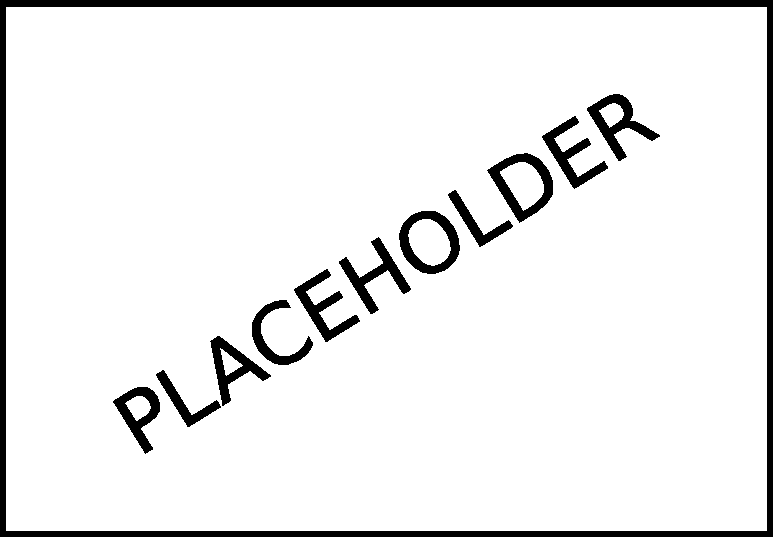
\includegraphics[width=0.8\textwidth]{gfx/placeholder}
    \caption{TODO}\label{fig:code-gen}
\end{figure}

\section{Generating ROS artefacts}
An automatic programming approach is a collection of rules and methods to transform an initial description to a different, more complex output. Therefore, even before the definition of the transformation itself it is necessary to define the input and the output of the process. In Chapter~\ref{ch:Modelling} we described in details a collection of meta-models that can be used to define ROS architectures using AADL in combination with a data modelling language (\ie, ANS.1 or JSON schema). A model compatible with this meta-models is the starting point of our automatic code generation process. Since the expected output of the entire process is a complete working architecture, the model alone is not enough as an input. To have a functioning architecture, the designer needs to pair the model definition with the implementation of the node inner functionalities; this can be done by using AADL properties. A ROS complete architecture is composed by multiple elements: existing nodes run as external resources, new nodes and messages created by the developers, launch files to organize the architecture, parameter profiles to configure the system. All these elements are  captured by the model, and can be automatically generated by our process. First, the automatic programming system creates the source code for the new custom nodes, the target language is C++. ROS supports multiple languages, mainly C++ and Python, Lisp is officially in the list but rarely used, and there are experimental libraries for Java and Lua. From the ROSwiki, \textit{rospy} (\ie, the Python implementation of ROS) is suggested as the approach that promotes implementation speed (\ie, reduced development time) over runtime performance, and it is designed specifically for fast prototyping, testing and lightweight implementations (\eg, configurations and initialisations), while \textit{roscpp} (\ie, the C++ implementation of ROS) is considered the main library, and it is designed with a focus on high performances and runtime speed. Since the output of the automatic programming is at the end of a long process involving a model-based design and carefully development components, we decided to use \textit{roscpp}, and therefore C++, as the target library to achieve the most efficient and robust implementation. Since C++ is a compiled language, the system will automatically generate all the necessary files to build the node executables; if the designer specify all the necessary information in the model (\ie, source code of the functionalities), the final output of the automatic programming process will be ready to compile with no intervention required. The automatically generated code will be placed in the correct package structure expected by ROS, together with any custom message, service or action file. This covers everything necessary for the execution of single nodes, to put them together in an architecture it is necessary to create launch files. In launch files, the designer specifies the instances of the nodes and how they are connected, by renaming all the necessary topics, and configured, by including configuration files. The topology of the architecture can be automatically extracted from the model and converted in a launch files, and the parametrisation defined using a data modelling language (\ie, ANS.1 or JSON schema) can be converted in the YAML description used by ROS. Moreover, in launch files existing nodes are included in the architecture and connected to the rest of the topology.

Figure~\ref{fig:code-gen} summarises the complete process. Our automatic programming approach requires as input a model defined in AADL, completed by a data description using ASN.1 or JSON schema, and specialised via properties to include functionality-specific source code. When all these conditions are met, the process provides as an output a collection of automatically generated and compilation-ready ROS nodes, their associated communication files (\ie, messages, service and action files) and the necessary launch files to run the architecture. A fully complete model creates an architecture that only needs to be compiled and run.

\begin{figure}[t]
    \centering
    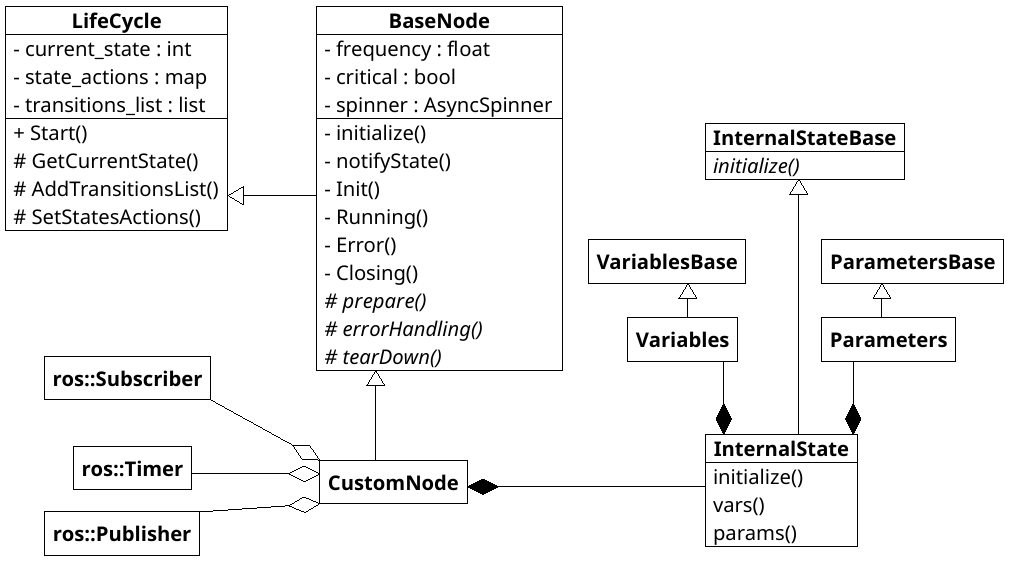
\includegraphics[width=\textwidth]{gfx/class}
    \caption{TODO}\label{fig:node-class}
\end{figure}

\section{Engineered ROS node}
\label{sec:ros-node}
Differently from other middleware or frameworks, ROS does not constrain the developer on the structure of the components; it was designed to be maximally flexible following the mantra: ``\textit{we don't wrap your main()}''. While this approach certainly contributed to the popularity and growth of ROS as a middleware and de facto standard for robotics, at the same time it created a very heterogeneous landscape for ROS nodes. Some of them are well designed, rich in functionalities, robust and configurable, others are cobbled together for a prototype and then used as legacy code for one single core functionality. Often this second category is created by experts in a specific field (\eg, vision, control, manipulation, \etc) that lack the necessary programming and software engineering skills and knowledge to develop a well-designed and robust node. With our approach we are targeting specifically this category of developers, that posses the expertise to contribute to the robotic community, but are discouraged by the programming required.

Since ROS does not impose any structure for the node, the simplest approach for automatic code generation would be to target an essential node, covering the minimum functionalities required to run it. There are few advantages in this approach: easier to implement code generator, simpler and more readable output, an implementation closer to what the developer knows. However, such a direct approach would have significant downsides: a lax relationship between the node and its model, lack of advanced functionalities that can be hidden in the automatic programming approach, less flexibility of the implemented node, more work left to the developer (\eg, testing, debugging, performance evaluation, \etc), more tampering by the developer with the basic structure of the node, no real benefit between a handcrafted and an automatically generated node. For all these reasons we decided to created an engineered base node that can be used as a reference and starting point for automatic code generation.

%TODO may not be simplified in the final version
Figure~\ref{fig:node-class} shows a simplified UML diagram of a custom node based on the engineered ROS node. Immediately, it is possible to recognise three main components: \textit{LifeCycle}, \textit{ROSNode}, and \textit{InternalState}. Each of them represent one of the main characteristics captured by the engineered node. The \textit{LifeCycle} implements an internal state machine that controls the evolution of the node. The \textit{ROSNode} is the core implementation of the node, capture all the ROS-related functionalities and management procedures. The \textit{InternalState} capture all the developer-defined parameters and variables necessary for the correct execution of the node.

\subsection{Life cycle}
When working with component-based approaches, it is important to define a recurring and consistent behaviour of the component, in the case of robotic components it is even more important, since they often operate with strict timing constraints and implement critical functionalities. In Section~\ref{sec:ros-in-aadl}, we presented how a life cycle of a node can be modelled in AADL, and how it can be used to guide the initialisation, configuration and execution of a component. To capture the same behaviour in the engineered node, we developed the \textit{LifeCycle} class to define the evolution of the node. While various implementations of state machines in C++ already exists, a very popular one has been around for almost 20 years\footnote{https://www.codeproject.com/Articles/1087619/State-Machine-Design-in-Cplusplus-2}, we opted to create a stripped down version that trades some functionalities for simplicity, understandability, and modern development approaches. The result is a very lightweight state machine, that supports dynamically defined states and transitions and it is completely ROS-independent.

To maintain the generality of the implementation, the class itself does not specify any state or transition. It only defines an empty enumeration that the subsequent classes can extend to define their own states. The valid transitions are defined as a list of pairs, going from one state to another, as for the states, the list is created by classes extending or using the state machine. The last initialisation step before running the state machine is to bind each state to a function. In practice, the binding is done by creating a map with the state as the key and a \texttt{std::fuction} as the value. Class template \texttt{std::function} is a general-purpose polymorphic function wrapper, it can be assigned to any callable target (\eg, functions, lambda expressions, pointers to member functions, \etc), this makes this approach particularly flexible and not bound to any specific implementation. When the initialisation is complete, the state machine can be started, the initial state is the one defined in the constructor, but there is no specific definition for a termination state. At each execution loop, first, the state machine execute the function bound to the specific state, then, it checks if there is a valid transition waiting to be performed, if there is one, the loop repeats and a new state-bound function is executed, otherwise the state machine has reached a final state and the execution terminates. While the list of all possible transitions is defined during the initialisation phase, each specific change of state is defined at runtime in all the state-bound functions. This is necessary, for example, to distinguish between a successful component initialisation that goes from an initial to a running state, to an unsuccessful one that would take the component to an error state. In practise, at the end of each state-bound function, the developer needs to specify the next state depending on the current outcome of the execution, then the state machine will check if the transition is valid (\ie, it is in the transitions list) and execute it. Mirroring the model presented in Section~\ref{sec:ros-in-aadl}, the engineered node supports five different states: initialisation, running, error report and closing. How they are implemented, what is their role and which ROS functionalities they evoke will be detailed in the next section.

\begin{figure}[t]
    \centering
    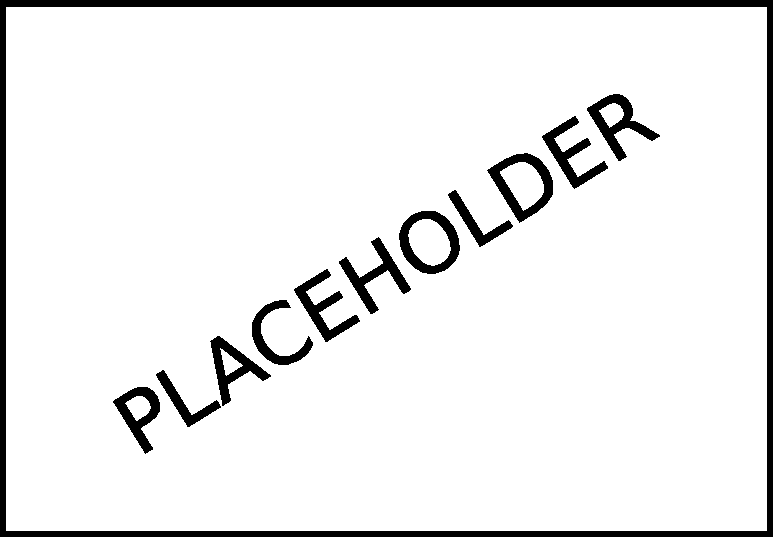
\includegraphics[width=0.8\textwidth]{gfx/placeholder}
    \caption{TODO}\label{fig:state-machine}
\end{figure}

\subsection{ROS node}
The core implementation of the engineered ROS node is in the \textit{ROSNode} class, here the life cycle is defined and materialised, and all the basic ROS-related functionalities are implemented. By defining this class, we can streamline the development process of a component by hiding the base initialisation procedure of a ROS node, create a well defined structure the developer can follow, and enhance the base implementation by adding additional functionalities (\eg, error detection and state report). The \textit{ROSNode} class extends directly the \textit{LifeCycle} class, therefore, the first implementation step is to define the states, the valid transitions and method bound to each state. Figure~\ref{fig:state-machine} presents the complete definition of the internal state machine, this mirrors the description provided in Section~\ref{sec:ros-in-aadl}. Each state is bound to a specific method of the class, and it implements a core functionality of the node.

\paragraph{Init} This method is bound to the initial state of the node (\ie, \texttt{ST\_INIT}). It is defined as a two-steps process and all the initialisation procedures of the component are implemented here.

The first step is a common initialisation that applies to every node, it sets up the ROS environment and defines the asynchronous spinner\footnote{http://wiki.ros.org/roscpp/Overview/Callbacks and Spinning}. In Section~\ref{sec:ros-in-aadl}, we modelled the ROS node with a external port to communicate the current state of the node after every transition, in this phase of the initialisation, the base node create the connection with the ROS service in charge of receiving this notifications. In ROS, a client can register to a service even if the server is not active, all the communications are lost until the service is finally started. This behaviour is not a problem for a status notification system, since it is meant to exist only to supervise the general evolution of the internal life cycle of the node. Nevertheless, our aim is to create a flexible base node that can adapt to different situations, thus, we defined an extra configuration property for the node, the developer can initialise the node as \textit{critical}. When a node is critical, instead of just starting the status notification service, the initialisation procedure will wait until the service is up, and then registers to it. In this way, an external supervisor node in charge of monitoring all the critical nodes can trace the entire evolution of their life cycles and act accordingly if something does not behave as expected. After the general initialisation procedure, the first action is to externally notify the state of the node, again the notification method itself behave in a different way for critical and non-critical nodes. To save bandwidth and reduce the number of requests, non-critical nodes notify their new state after a transition only if it is different from the previous one, in other words, they do not notify transitions on self-loops. Critical nodes are meant to be constantly monitored by the supervisor, therefore they notify their state after every transition, basically, in this case, self-loops are used as a way to measure the liveness of the node.

If the basic initialisation is completed successfully, the second step of the set up of the node is activated. An unsuccessful outcome is considered a critical failure and the node is instantly shut down. The second part of the initialisation is an abstract method not implemented in the \textit{ROSNode} class (\ie, the \textit{prepare} method) and it is meant to be used by the child class to define any node-specific initialization procedures. The developer can use this method to fill parameters and variables with their initial values, set up publishers and subscribers, or perform any other special initialisation (\eg, activate hardware connections, pre-fill data structures, \etc). If this preparation phase is completed successfully the method will trigger the transition to the main execution state. Differently from the base initialisation, an unsuccessful preparation phase will trigger a transition in error state. This is because we cannot anticipate what kind of procedure the developer will implement in this second part of the initialisation, therefore issues in this phase may be resolved in a specific error management procedure and lead to a successful initialisation.

\paragraph{Running} A complete and successful initialisation will transition the state machine in the \texttt{ST\_RUNNING} state, and this is the method bound to it. Since the engineered ROS node is built around an asynchronous spinner, most of the ROS-related functionalities (\ie, checking subscribers, services and timers) are executed in a separate thread, hence this method only needs to check for errors or node termination. When the node is working with no issues, the \textit{Running} method is just a low-frequency (\ie, 1 Hz) repeating self loop, two things can change this condition: first, one of the asynchronous activities (\eg, a subscriber callback) sets an error flag, or second, an external signal triggers the shutdown procedure. In the former case, this method interrupts its self loop and trigger a transition to the error state, in the latter, it receives the signal and changes the current state of the life cycle to shutdown. When the node is initialised as \textit{critical}, the behaviour of the \textit{Running} method does not change, however, the state notification happens at every self loop instead of only after the first transition. Given the fundamental functionalities implemented in this method, the developer cannot directly modify it, however it is possible to change the frequency of the self loop. Given the structure based on the asynchronous spinner, changing the frequency will not influence the behaviour of any ROS-related functionality, but it can change how fast the node reacts to errors or terminations; specifically, the higher the frequency the shortest will be the time between the generation of errors and interrupts and their detection. Changing the frequency of the self loop it is also useful to monitor the liveness of critical nodes. 

\paragraph{Closing} As any other process, ROS nodes can be closed by sending a termination signal (\ie, SIGINT). Normally, they already implement a handle to capture the signal and force a shutdown of the node, in the engineered node we replace it with our own version. Our handle does not perform any shutdown procedure, it just capture the signal and sets a flag; this flag will cause the \textit{Running} method to trigger a transition to the \texttt{ST\_CLOSING} state.  In this method bound to the state is where the actual shutdown procedure happens: first, it triggers a final state notification, so a potential supervisor knows that the node is shutting down, then it execute a custom \textit{tearDown} method, and finally it shuts down any ROS-related functionality. The \textit{tearDown} method is the shutdown counterpart of the \textit{prepare} method of the initialisation. It is abstract and not implemented in the base class, any child class extending \textit{ROSNode} will implement it with their own specific shutdown procedure. This is done to let the developers gracefully close existing connections (\eg, device drivers), propagate the shutdown to other nodes (\eg, critically dependant components), or provide additional shutdown notifications (\eg, specific logging systems). Since this is the terminal state of the life cycle, this method does not implement any transition.

\paragraph{Error} Natively, ROS does not provides any system to manage errors during the execution of the node. In our engineered node, we created an extensible structure to identify, detect and react to errors. The \textit{ROSNode} class defines an enumeration with few predefined error codes, they cover some common issue that may happen during the normal functioning of a node. They are:
\begin{itemize}
\item \texttt{PARAM\_ERROR}: this is a typical initialisation error, when a necessary parameter is not found in the parameter server. The node cannot run correctly when partially initialised, a way to handle this error is to wait until the parameter is available and then restart the initialisation procedure.
\item \texttt{SUB\_FAILED}: one of the subscribers of the node fails. This may compromise the entire node (\eg, set-point subscriber for a control node) or just disable one of its functionalities (\eg, a multiplexer missing one of the inputs). Depending on the situation this may or may not require the shutdown of the node. 
\item \texttt{PUB\_FAILED}: one of the publishers of the node fails. As for the subscribers, this may be very impactful (\eg, a planner that cannot publish the result) or a minor inconvenience (\eg, a visualisation topic not initialised), and therefore could prompt a shutdown of the node.
\item \texttt{INVALID\_MESSAGE}: This is an error that can be triggered during a subscriber callback or before publishing a message. A message has an unexpected value (\eg, negative distance, out of bound acceleration, empty path). Sometimes malformed messages are inconsequential, and the error handler will just record them, in other cases they can be hazardous and require to halt the node execution. 
\end{itemize}

These error codes are mostly related to the correct execution of ROS functionalities, on top of these, the developer can extend the enumeration and define his own error codes, to cover problem-related corner cases. 

At any moment during the normal execution of the node, the developer can use the \textit{faultDetected} method to notify one of the possible error codes. After the initialisation process or during the \textit{Running} self loop, if any error code is set, the system will transition to the  \texttt{ST\_ERROR} state. The \textit{Error} method is bound to this state, during its execution, first it notifies the state transition, to let any potential supervisor know that the node is in an error state, then it calls a method to handle the error, finally, after \textit{errorHandling} returns, if the error code is still set, the error is unsolvable and the node transition to the \texttt{ST\_CLOSING} state, otherwise, the node can go back to normal execution. The \textit{errorHandling} method is similar to the abstract method used during the initialisation and closing phases, as before, it is an abstract method that the developer can extend in the child class to manage any specifically defined error codes. Differently from the previous two, it is not a pure abstract method, since we provide a basic implementation in the \textit{ROSNode} class to manage the four already defined error codes. The developer can decide to reimplement completely the method (\eg, complex nodes with articulated initialisation procedures), run it alongside the existing one (\eg, few problem-related corner cases), or skip error management and leave only the already defined implementation (\eg, simple node requiring minimal definitions).

\subsection{Internal state}
Components are meant to be reusable through composition and parametrisation. The computation graph of ROS combined with our model-based approach ensure the composability, by providing deployment-time rewiring and decomposing components functionalities. On the contrary, parametrisation is not embedded in the design of the nodes. ROS provides various system-level tools to manage parameters: a centralised system to store and collect parameters (\ie, the parameter server), the corresponding APIs to fetch and set them, and a system to dynamically change parameters in real time. However, how to integrate them in the component is left to the developer. The result is parametrisation is often ignored or misused. Parameters are uncategorised and mixed between functionalities, modified during execution creating inconsistencies, defined conceptually but then hard-coded as constants in the implementation. This issues prompted us, originally, to exploit data modelling languages to capture the parametrisation of the component, and, in the engineered node, to design a separate class to encapsulate the parameters of the node.

Parameters are the external-facing part of the internal state of the component, they codify a specific configuration defined before execution; variables, on the opposite, are internal-facing, they evolve with the node and exist only in the time frame of its execution. As mentioned at the beginning of this section, ROS does not provide any structure to support the internal state of the node, in the case of the variables, it means there is no predefined way to safely store and share between callbacks the information extracted and derived from messages. Normally, there are two approaches used when developing ROS nodes, one is for traditional imperative implementations, where variables are declared as global and shared between callbacks, the other wrap the entire node in a class, it uses methods as callbacks and attributes for variables. While this approaches are not inherently wrong, they have significant downsides. They reduce the portability of the node design by removing the distinction between ROS-specific (\eg, declaration of publishers and subscribers) and problem-specific (\ie, the necessary logic to implement the functionalities of the node) implementations, they are harder to debug since they are not encapsulated and may have unpredictable side effects, they are more difficult to extend and modify since they do not present a common interface. Our solution is to create an overarching class encapsulating both parameters and variables, and present a single interface that the developer can use to access, modify, share and store the internal state of the component.

As visible from Figure~\ref{fig:node-class}, the internal state of the node is built using a hierarchical approach. The superclass is called \textit{InternalStateBase}, it has two members: a structure for variables of type \textit{VariablesBase} and a constant structure for parameters of type  \textit{ParametersBase}. Parameters are defined as constant, this means that after setting their values during the initialisation phase, it is guaranteed they will not change. An exception to this is when the node implements a dynamic reconfigure system, in this case there is a special callback in charge of managing the parameters and changing them according to an external control panel. In general, by defining the structure as constant it is possible to limit any modification of the parameters to specific procedures, and avoid unintentional modifications using compile-time checks. Both the parameters and variables structures are defined as shared pointers, this pointer-based declaration gives us the ability to treat each structure as a single entity, while, at the same time, avoiding useless and memory-consuming copies when accessing them in external procedures. The superclass has only one method, a pure abstract initialisation method that the developer has to implement in the child class; this is designed to force the developer to initialise all the parameters in the same location and to set an initial value to all the variables. To increase the flexibility of the base node, the internal state is not declared directly in the \textit{ROSNode} superclass, the developer can extend \textit{InternalStateBase} to create his own internal state class and declare it in the custom node. To better exploit the structure provided by the superclass, the developer can extend the parameters and variables structures, to define all the problem-specific details.

\section{Custom ROS node}
In Section~\ref{sec:ros-node}, we presented the engineered node as the starting point for the automatic programming process, however, the classes defined are perfectly suitable to be used directly by a developer to create their own node. In this section, we will present how a custom node can be implemented using the engineered node as a starting point, using the same approaches and structures the automatic code generator would create.

Since it is an independent class used by the rest of the node, the first step should be the definition of the internal state, and in that, the developer has to start from the definition of his own variables and parameters structures. Although the two base structures do not provide any functionality, it is ideal to extend them and exploit a polymorphic approach to define the internal state. The automatic code generator extends them and adds constructors to initialise the instances to their default, for parameters, and initial, for variables, values. The \textit{InitialStateBase} class exists to provide an unified interface between the node and its internal state, therefore, following the concepts of information hiding used in object-oriented programming, it is necessary to implement accessors for both parameters and variables. Since we are working with pure data structures declared as shared pointers, the most elegant approach is to define accessors for the entire structures and let the developer use directly the fields. To complete the definition of the internal state, it is necessary to implement the abstract initialisation method. A developer can create any complex initialisation, but in our automatic programming approach, we delegate the parameters set up to the core node functionality and use a copy constructor, while for the variables we invoke the constructor with no parameters defined in the structure.

After completing the definition of the internal state, a developer can move to the implementation of the node itself. The engineered node wraps all the main ROS-related functionalities in a single class, to implement the custom node the developer has to extend the \textit{ROSNode} base class. In the custom node class declaration three abstract methods are overridden from the superclass: \textit{prepare}, \textit{tearDown} and \textit{errorHandling}. Additionally, all the callbacks related to subscribers, services, timers and actions are defined as class methods. Since the class is the container of all the ROS-related code, the timer, publisher, subscriber, client, server and action objects are all declared as class members. Lastly, to complete the class definition, it is necessary to declare the internal state instance. These are all the methods and attributes that are necessary to implement the child class as an extension of the \textit{ROSNode} base class, and to cover all the fundamental ROS functionalities. When using the code generator only these methods and attributes will be automatically created, however, there is no restriction on the complexity of the class and a developer can declare all the additional helper methods and attributes necessary to ensure the proper functioning of the node.

As introduced in Section~\ref{sec:ros-node}, the \textit{prepare} method is meant to contain all the node-specific initialisation procedures. Here the code generator will create all the necessary calls to collect the parameters from the ROS parameter server and initialise the internal state of the node by setting the initial values of the variables. Moreover, callbacks of subscribers are initialised, publishers and services are advertised, and timers are set. At the end of this method, the node is ready and fully functional. Since it is abstract, the developer needs to implement the \textit{tearDown} method, here, all the necessary procedures to gracefully shutdown the node are executed. ROS manages all the connections transparently with respect to the end user, therefore, in a generic node there is no need for any particular shutdown procedure. If not specified otherwise in the model, the automatic code generator fills this method only with an output message to notify the system that the node is shutting down.  The last method that is necessary to implement to complete the definition of the child node as an extension of the base class is \textit{errorHandling}. All the structure to manage errors is not ROS-related and it is defined by us in the base class, since this is an extra functionality not necessary for the basic operation of the node, we already provide a simple handler that can be called directly and manages basic initialisation errors. However, if the developer wants to exploit the error management system, he can define his own error codes in the class by extending the enumeration defined in the \textit{ROSNode} superclass, and implements his own version of the \textit{errorHandling} method. Potentially, a developer could implements an extension of the internal life cycle of the node, where instead of a single error state there are multiple error states, each for a different category of problems. This can be done by extending state enumerator, binding new methods to the new states, and add all the necessary transition in the state machine. This is possible because by overriding the \textit{errorHandling} method, not only the developer can develop his own error management procedures, but he can change how the internal state machine evolves from the \texttt{ST\_ERROR} state. Without any specification in the model, the code generator will not override this method and use the implementation provided in the base class. While it is possible to specify in the model an implementation for the method itself, if the developer wants to change the life cycle of the node, he needs to do that by modify directly the source code, since the modifications are too radical and in depth to be managed by an automatic programming system.

The last step to complete the implementation of a custom node is to define the logic related to the subscribers, timers, or actions callbacks. As mentioned at the beginning of this section, all the callbacks are defined as methods of the child class; ROS already defines the signature for all the callbacks, hence the developer only needs to implement them. He can read parameters from the internal state and store the output of processing in the variables structure. Practically, there is no issue in implementing the logic directly in the callbacks, however, with our automatic programming approach we try to push as much as possible the separation between the problem-specific and the ROS-related implementation. The automatic code generator creates a function call for each callback using the structure defined in the model as a reference. The functions have access to the parameters and variables structures and to the message, but their entire implementation is completely independent from the node. This function can be used as a bridge between ROS and a domain-specific library and can be easily tested and debugged without the need of running the node. With the addition of the logic the implementation of the custom node is complete. Of course, since this is a C++ implementation, the developer needs to create all the necessary configuration files to build the executable. With the automatic programming approach, all the necessary file are generated, and the developer only needs to add additional sources that were not specified in the model.

\section{Two-steps code generation}
Now that we have completely defined the input, a complete model description defined in AADL following the meta-model presented in Chapter~\ref{ch:Modelling} combined with data modelled using ASN.1 or JSON schema, and the output, the engineered ROS component implementing advanced functionalities and a list of approaches to implement a custom node, we can describe all the necessary transformations to convert the collection of model to a working architecture. In our toolchain, we adopted a two-steps approach, first a model-to-model transformation that converts the  input AADL model to an intermediate XML-based representation, then a model-to-text transformation to automatically generate ROS-compatible C++ code.

While AADL is popular in some specific fields (\eg, space applications, automotive and embedded hardware), it is a niche language, therefore there are only few options in terms of tools and support. In particular, there is only one maintained and open-source AADL model processor that supports model checking, parsing and code generation: Ocarina. As presented in Section~TODO, Ocarina is written in Ada and provides multiple functionalities (\eg, parsing, model analysis, schedulability analysis, \etc), but mainly it is a parser and code generator. With its frontend/backend structure it separates the parsing and syntax analysis of the AALD model (\ie, frontend) from the code generation of a specific target (\ie, backend). This means that a developer could implement its own backend to exploit the parsing capability of Ocarina to create his own code generator. In theory, we could have used this approach to create directly a code generator completely implemented as a backend, but we decided to use Ocarina only to create an intermediate representation.

There are multiple reasons behind this choice. First of all, not only Ocarina is implemented in Ada, but is follows the Ravenscar profile, this is necessary because some of the code generation targets are certified for safety-critical hard real-time applications, therefore the toolchain itself needs the same certification. The Ravenscar profile imposes some restrictions on the already challenging Ada language, making the development and maintenance of a new backend a difficult and time-consuming task. By using an intermediate representation we can implement the most challenging part of the code generation (\ie, ROS source code) with our preferred approach. Additionally, using an XML-based language, that we called AAXML, creates an intermediate artefact that can be used as a starting point for code generation, but also as the output of a different AADL parser. Ocarina is an independent project that we do not control directly, therefore we cannot base our entire toolchain on a technological solution that could disappear or change drastically. Lastly, a two-steps approach makes the entire toolchain more flexible, for example to extend the code generator to support ROS2 or a different framework, or to include additional models (\eg, a specific language to describe the component behaviour). There is one final, more practical reason, to adopt a two-steps approach and instead of generating directly ROS/C++ code, Ocarina already implements a backend that uses XML as a target. Unfortunately, the existing XML backend is currently non functional and not maintained, it was developed as a low-priority approach in an effort to create a bridge between AADL and a possible XML-based representation. Nevertheless, we used it as a guideline to create our own backend from scratch.

\subsection{From AADL to AAXML}
This is the first step of the code generation approach, it is a model-to-model transformation, since the original structure of the AADL model is preserved but converted in an XML-based representation called AAXML. The Ocarina frontend provides two output that can be used by the backend: an abstract semantic tree, this guarantee correctness of the syntax and semantic of the model, and an instance tree, this is the result of the instantiation process; both of them are used by the backend. To implement the \textit{aaxml\_ros} backend, we followed the structure already established by Ocarina, with few modification to make the toolchain more suitable to the needs of a robotic system. First the backend needs to be registered to the frontend, so it can be called by the toolchain, after this simple initialisation phase, the automatic code generation process can start; it is a recursive approach that  analysing the root system of the model and goes through subcomponents, features, connections, and properties. In the default Ocarina implementation of a backend, only a single system can be parsed by the toolchain per call, but since in our model the hierarchy of AADL systems represents the deployment configuration of the architecture (\ie, launch files in ROS), we decided to modify the backend to parse all the root system component (\ie, system that are not subcomponents of other systems) to be able to generate all the necessary launch files at the same time.

\paragraph{components} As mentioned before, the code generation process is recursive, it always starts from a component. A component is mostly characterised by its subcomponents, ports and connection, however, few details can be extracted directly from it and converted to AAXML. The \textit{name}, an unique identifier of the actual instance of the component, necessary when there are duplicates coexisting in the same architecture. The \textit{type}, the reference to the specification of the component, depending on the level of specification it can be an interface or a complete definition. The \textit{category}, this attribute specify the AADL type (\eg, process, thread, system, \etc) associated with the component, it is guarantee to be compatible with the container component by the syntactic and semantic analysis done by the frontend. The \textit{namespace}, it specifies the package containing the component, while this seems a superfluous information, it is extremely important when referencing component not defined in the same package of the system. The subcomponents list, AADL has a hierarchical structure and Ocarina manages it using a recursive approach, this list is used to perform all the recursive call and complete the traversal of the tree.

Listing~\ref{lst:comp-aadl} shows a small example of a system containing a single process as subcomponent, this is the minimal AADL architecture that we can model and instantiate. In Listing~\ref{lst:comp-aaxml} presents the AAXML counterpart of the model, where the properties described are encoded in an XML-based format. In this minimal structure, no information is lost when converting the model from AADL to AAXML.

\begin{lstlisting}[frame=tb,caption={TODO caption},label=lst:comp-aadl]
system root_system
end root_system;

system implementation root_system.impl
  subcomponents
  main_process: process custom_process.impl;
end root_system.impl;
\end{lstlisting}

\begin{lstlisting}[frame=tb,caption={TODO caption},label=lst:comp-aaxml]
<system>
	<type>root_system.impl</type>
	<category>system</category>
	<namespace>aadl_xml</namespace>
	<subcomponents>
		<component>
			<name>main_process</name>
			<type>custom_process.impl</type>
			<category>process</category>
			<namespace>aadl_xml</namespace>
		</component>
	</subcomponents>
</system>
\end{lstlisting}

\paragraph{Features} The subcomponents list is one of the defining characteristics of a component, the other is the set of features. They define the frontier between the component and the external environment, moreover, when working with interface-only definitions (\eg, existing ROS nodes), they are the only element characterising the component. For these reasons it is important to capture all the necessary information when converting the model from AADL to AAXML. Features have a list of characteristics that are mandatory and are necessary to specify them, and others that optional. First of all, it is necessary to identify the type of feature, AADL categorises them in two main groups: accesses (\ie, subprogram, data and bus) and ports (\ie, data, event and event data); this is captured by the \textit{category} tag. By defining the \textit{type} it is possible to specify the specific subcategory of a port (\eg, \textit{event\_data}), for accesses there is no need for specialisation since the component they are connected to determinates their  specific subcategory. Another attribute that is unique to ports and not necessary for accesses is the \textit{direction}, since ports can define a specific ingoing, outgoing or bidirectional communication. While in the model it is necessary to specify if a feature provides or requires access, this specification can be dropped in this conversion since it is important only to define the topology of the architecture, which is already checked by the frontend. This covers all the mandatory definitions for a feature, additionally, it is possible to specify the data type of the feature. Since the data is a component, we need two information to identify it: the package and the type. While subprogram and bus accesses target a subprogram or bus instead of a data component, the procedure is the same since they are identified by their type and package.

Listing~\ref{lst:feature-aadl} show the interface model of the component included in the system presented in Listing~\ref{lst:comp-aadl}. It defines a single event data port exchanging messages with a specific data type. Given this definition the AAXML file can be extended as shown in Listing~\ref{lst:feature-aaxml}, the \textit{features} tag is a child of the \textit{component} tag, while this replicates the feature information in multiple places in the file, it also streamlines the code generation process in the next phase.

\begin{lstlisting}[frame=tb,caption={TODO caption},label=lst:feature-aadl]
process custom_process
	features
		a_port: out event data port pkg::some_data;
end custom_process;
\end{lstlisting}

\begin{lstlisting}[frame=tb,caption={TODO caption},label=lst:feature-aaxml]
<component>
	[...]
	<features>
		<feature>
			<name>a_port</name>
			<direction>out</direction>
			<type>event_data</type>
			<datatype>some_data</datatype>
			<datatype_namespace>pkg</datatype_namespace>
			<category>K_PORT_SPEC_INSTANCE</category>
		<feature>
	<features>
</component>
\end{lstlisting}

\paragraph{connections} When dealing with connections we move outside the scope of a single component and we have to consider the interaction of multiple objects. For this reason, connections are defined, both in AADL and in AAXML, in the container, and they can connect two components in the same subcomponents set or a component and a frontier feature (\ie, a feature defined on the frontier of the container component). First, there is a list of characteristics referring directly to the connection itself. The \textit{name}, an unique identifier of the connection. The \textit{kind}, a mapping in AAXML of the original Ada node kind, currently the only possible value is \texttt{K\_CONNECTION\_INSTANCE}, however, we decided to include it in the AAXML file to support future extensions. The \textit{category}, as for features, connections may involve ports or accesses, this property specifies the type of the connection, it can be: \texttt{CT\_PORT\_CONNECTION}, for connection between two ports, \texttt{CT\_ACCESS\_DATA}, when connecting an access to a data component, or \texttt{CT\_ACCESS\_SUBPROGRAM}, when modelling a connection representing a remote subprogram call. Since connections are meant to describe the interaction between component, they carry information related to both components at the limits of the connection. Each description has a subsection called \textit{port\_info}, it includes the name of the source and the destination features, and the name and the type of the parent components.

Listing~\ref{lst:con-aadl} shows the modelling of the implementation of a system where two processes are connected, one with an output port and the other with an input port. Listing~\ref{lst:con-aaxml} presents how this connection is mapped on the AAXML file, since the system is the root of the hierarchy, the \textit{connections} tag is defined directly as a child of the root \textit{system} tag.

\begin{lstlisting}[frame=tb,caption={TODO caption},label=lst:con-aadl]
system implementation root_system.impl
	subcomponents
		cmpA: process pkg::processA;
		cmpB: process processB.impl;
	connections
		con1: port cmpA.out -> cmpB.in;
end root_system.impl;
\end{lstlisting}

\begin{lstlisting}[frame=tb,caption={TODO caption},label=lst:con-aaxml]
<system>
	[...]
	<connections>
	<connection>
		<name>con1</name>
		<kind>K_CONNECTION_INSTANCE</kind>
		<category>CT_PORT_CONNECTION</category>
		<port_info>
			<source>out</source>
			<dest>in</dest>
			<parent_source>processA</parent_source>
			<parent_source_name>cmpA</parent_source_name>
			<parent_dest>processB.impl</parent_dest>
			<parent_dest_name>cmpB</parent_dest_name>
		</port_info>
	</connection>
	</connections>
</system>
\end{lstlisting}

\paragraph{properties} In AADL, properties can be applied to every element in the model, moreover, in the definition of our meta-model, we introduced their importance in specifying components. Properties are such an important element of the languages, that additionally to all the already existing definitions, the designer can define his own set of new properties. Given their ubiquitousness, each AADL category has a set of general properties, plus specific ones, plus all the custom defined, the process of adding them to the AAXML file can happen at every point during the parsing of the tree. All properties defined in the model have at least two fields: the \textit{name}, the unique identifier of the property as defined in the language definition or in the property set, and the \textit{value}, the actual value of the property assigned by the designer in the specific instance of the model. Each property has a type (\eg, number, string, \etc), that is checked by the frontend for consistency but not replicated in the AAXML file, additionally, in AADL it is possible to define the measurement unit of a specific property, if present, it is included in the translated model using the \textit{unit} tag. Default (\eg, \textit{Period}) and custom (\eg, the \textit{Default\_name} of a topic) properties are managed in the same way, with the exception of the name of the property set containing the custom defined properties; it is included in the AAXML file using the \textit{namespace} tag. In AADL it is possible to set properties at any point in the model, this means that in the property section of a component it is possible to reference every property of its internal parts (\eg, features, connection, subcomponents,\etc) or, through dot notation, all the properties of the subcomponents. However, in AAXML, properties are defined in as direct children of the element owning them.

Listing~\ref{lst:pro-aadl} shows a definition of the implementation of a process component, it has a thread as a subcomponent and this thread has an output port on his frontier. As said before, it is possible, in the properties section of the process to specify both the properties of the subcomponent (\ie, \textit{Period}) and of the feature (\ie, \textit{Queue\_size}). Listing~\ref{lst:pro-aaxml} presents a portion of the AAXML file modelling the properties, while they were defined in the property section of the process, the \textit{component} tag in the listing references the thread, since it is the owner of both the feature and the \textit{Period} property. 

\begin{lstlisting}[frame=tb,caption={TODO caption},label=lst:pro-aadl]
process implementation componentA.impl
	[...]
	properties
		Queue_size => 1 applies to threadA.out;
		Period => 50 ms applies to threadA;
end componentA.impl;
\end{lstlisting}

\begin{lstlisting}[frame=tb,caption={TODO caption},label=lst:pro-aaxml]
<component>
	[...]
	<features><feature>
	<properties><property>
		<name>Queue_size</name>
		<value>1</value>
	</property></properties>
	</feature></features>
	<properties><property>
		<name>Period</name>
		<value>50</value>
		<unit>ms</unit>
	</property></properties>
</component>
\end{lstlisting}

\subsection{From AAXML to ROS/C++}
\label{sec:xml-cpp}
The second step of the code generation is a model-to-text transformation. Differently from the first step where the original AADL model was converted in a different format, here multiple models (\ie, AADL and ANS.1 or JSON schema) are combined to create code artefacts. In particular, the output of the code generation after this step will be a single ROS package that contains all the custom messages, services and actions (if they exists), the source code of all the nodes modelled combined with any already existing problem-specific implementation, all the necessary build and configuration files, and the launch files matching the deployment configuration specified in the model.





\textcolor{red}{
The code generator discussed in this work, takes the AAXML model produced by the customised back-end as input and translates it into a working ROS C++ environment, i.e., a set of one or more ROS packages equipped with all the necessary configuration files for compiling (e.g., the \textit{CMakeLists.txt} and \textit{package.xml} files, the custom messages and services, launch files, etc.). Each one of these packages also includes a programmatic list of all method interfaces declared by the developer within the model, making the output code application-specific.}

%We introduced two steps in our toolchain to exploit the already available XML parsers. 
The code generation module was developed entirely in Python 3, hence exploiting the \textit{lxml}~\cite{lxml} pythonic binding for the C libraries \textit{libxml2} and \textit{libxslt} (also integrating the XPath syntax~\cite{websiteXPath}), as XML Manipulation Toolkit.

For designing this code generator, we followed a Russian doll pattern, where elements call each others in chain until the final code is generated, as shown in Figure~\ref{fig:codegenerator-russiandollpattern}.

Each element in C++ to be generated has its own managing class in Python. For example, a variable in C++ is managed by a Python class which contains all the elements and the methods to represent the functionalities and properties of that C++ variable. The same goes for a C++ method, where a specific Python class manages it. Since a method can have variables as input, the corresponding managing Python class can contain an instance of the Python class dedicated to variables. Each of these variables has a specific type, which is managed by the \textit{type} class. When generating the C++ method code, the input parameter objects are triggered to generate their own code and together they cooperate to produce the complete method code.  Figure~\ref{fig:codegenerator-russiandollpattern} shows this exact example.

The entire code generation workflow is detailed throughout the remainder of this Section, accompanying each description with graph visuals.
%We will now go through the entire structure of the code generator detailing the code generator normal flow, summarizing with graphs the entire procedure.

\paragraph{Initialisation} The initialisation phase consists of some basic set-up instructions and the top-down reading of the AAXML tree. We used the \textit{XMLTags} module in Python for reading the tree, exposing all the AAXML tags produced by the Ocarina backend \textit{aadl\_aaxml} as a result. %Any change to the used tags in the first step of the toolchain is automatically reflected to the second step.
To accommodate for the main structure of AADL models being a \textit{system}, we also incorporated a \textit{SystemsManager} class in our code generator, to manage all the AADL \textit{system-level} components, represented instances of the Python \textit{System} class.

\paragraph{The System Loop} In AADL it is possible to define additional systems as system subcomponents. As a result, the code inspection and generation routine had to keep this factor into account. After the main system root (i.e., the outermost container) is retrieved, subsystems are lined up in a loop queue of type FIFO (i.e., First In First Out). Figure~\ref{fig:codegenerator-systemsloop} demonstrates how a \textbf{system loop} is formed: each highlighted block is the main actor of the following phases, where each system is analyzed and its code generated.
%This has to be treated accordingly by running the full code inspection and generation also over it; this chain can be as deep as one wants. 
%After gathering the main system root, namely the outer system, a loop queue is instantiated where new systems are added at the end, the already queued are popped one by one and examined. 
%This \textbf{system loop}. is shown visually in Fig.: the block highlighted is the main actor of the following phases, where each system is analyzed and its code generated.

\paragraph{Code Generation} The code generation process summarised in Figure \ref{fig:codegenerator-systemsloop} is quite straightforward. First, a new \textit{System} object is created, with all information relative to the current analyzed system (i.e., also including the launch file and the \textit{CMakeLists.txt} file ultimately required to compile and run the generated nodes). Both files are consistently updated by the code generator as the process goes on, this is necessary, since crucial information to be inserted these files (e.g., adding library dependency to ROS \textit{tf}) may only appear later in the code generation process.

Then, all the AADL processes in the \textit{system} are visited one at a time, in search for specific thread components that trigger the start of code generation. As thread components are identified by their type and, in this phase, a RegEx check is used to look for the target Python class matching the detected thread type. If a thread type is not recognised, it will simply be ignored and skipped by the code generator. In fact, in an AADL \textit{process}, threads can be associated to known types or marked as 'unknown'. This implementation strategy allows for the code generator to only look for supported parts, without limiting the completeness and expressive power of the input model. This may happen, for example, when modelling a sensor driver, which does not use publishers or subscribers to communicate with the hardware, but unique approaches, not identifiable by the code generator.

The currently supported thread types are six, reflecting the custom functionalities introduced in Section \ref{sec:transformation-rules}:
\begin{itemize}
\item{ \textbf{main\_loop.impl} identifies the main thread behind every single node. A node without this thread cannot work and it is skipped by the code generator.}
\item {\textbf{publisher.impl} identifies a thread with publishing capabilities. It is a generalised description, that needs some configuration parameters (e.g., message type, rate, topic name) to work properly and also a connection to specify where to send the published message.}
\item \textbf{callback.impl} is related to subscriber threads. As for its counterpart that publishes messages, a \textit{callback.impl} thread needs configuration parameters (e.g., message type, topic name) to be functional.
\item the \textbf{call\_pub.impl} thread receives a message in input and re-publishes it with some modifications. In a sense, it merges subscriber and publisher functionalities in one place.
\item \textbf{service\_provider.impl} indicates that the considered thread provides a service functionality
\item \textbf{timer.impl}, is the identifier used for threads that implement only timers and their callbacks.
\end{itemize}

%At this stage, the code generator starts looking for the known thread types and generates the relative code. 
The main thread is a required component for the process not to be ignored by the code generator. After the main thread is detected, the module analyses all the remaining threads. As flexibility is a requirement for future extension to new thread types, the thread libraries (i.e. the python classes \textit{Publisher}, \textit{MainThread}, \textit{Timer}) are imported at runtime only if used. This was achieved through the Python module \textit{importlib}. Defining and supporting a new thread type becomes then extremely easy and is done by simply extending the base class \textit{AADLThread} (which implements all said functionalities) and by adding an additional regular expression to map the newly-created class to its related thread type.

After all systems have been parsed and the queue is empty, the saving routine starts. In this phase, the launch file created at the very beginning is finally populated. Then, each node is saved and its executable name added to the \textit{CMakeLists.txt}, calling the instance of class \textit{CMakeLists} that manages it. Since the same node design can be reused inside the model, nodes sharing the same design, but with different functionalities, are generated. To overcome the problem of linking the correct node source to the node name in the launch file, after the node source is actually generated and saved, the equivalent entry in the launch file is updated if necessary. After the nodes and all their universe have been generated, it is the turn of custom messages and services.

\paragraph{Custom Messages And Services} In ROS it is possible to define a new custom message that relies on basic datatypes or on already existing ROS messages, and the same applies to services. To take advantage of these functionalities, we used a data modelling language called ASN.1. ASN.1 is an interface description language used to define data structures which can be easily serialised and deserialized. The code generator, is thus able to read and parse an ASN.1 description and to produce a working representation of a custom message or service, ensuring it is ROS-compatible. In ROS, message-only packages may exist, the code generator cover this case by creating the relative relative package with the \textit{CMakeLists.txt} during custom messages generation.

\subsection{Use Case: Publisher - Subscriber Example} \label{sec:use-case}

This section demonstrates a real use case of the customised Ocarina backend \textit{aadl\_aaxml} and code generator, when applied to a simple publisher-subscriber architecture. %The goal is to demonstrate that our toolchain is able to produce a good quality code.
We firstly introduce the publisher-subscriber model to then analyse its correspondence with the generated ROS package. To make the example more complete, we include the exchange of a custom message between the two nodes.

The AADL model represented in Listing~\ref{snippet:aadl_pub_sub_system}, shows a main system is called \textit{container} and its containing package \textit{pub\_sub}. Note that the latter package name will be reused as ROS package name. 
We refrain from reiterating all relevant definitions already introduced in Section~\ref{sec:background}, and discuss only the \textit{properties} associated to publisher-subscriber connection. Broadly, the publisher and the subscriber need to exchange messages on the same topic, where topics are identified by their name, e.g.,  \textit{``/pubsub"} in this case. The topic name is attached to the existing connection between the two, or, in other words, defined at the system level. In fact, placeholders for the topic should be specified within the process rather than as part of any other component of the system, in order to produce a functioning node.

% \begin{figure}[t]
% \centering
% 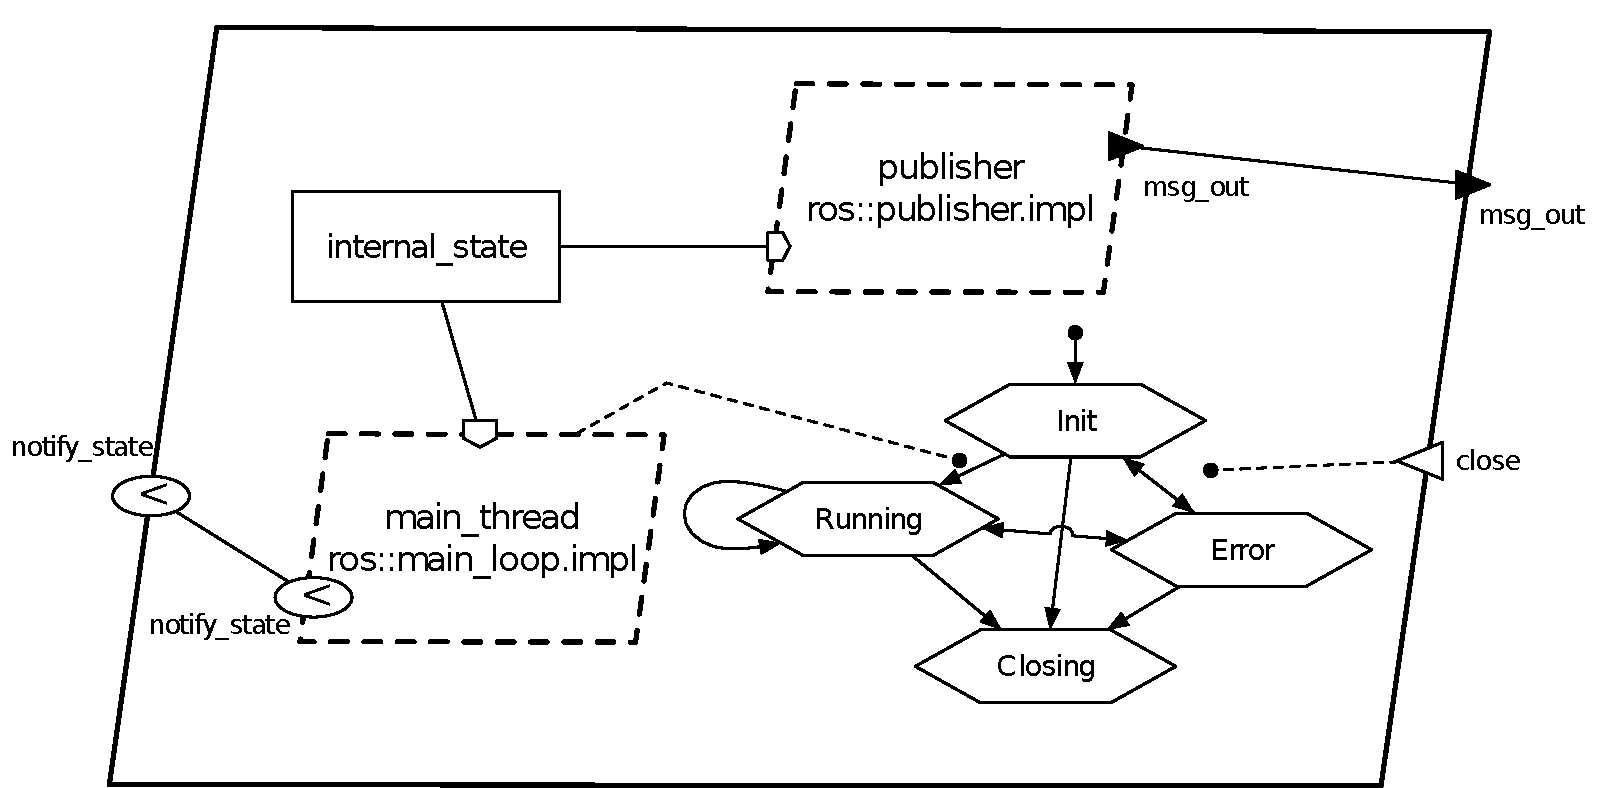
\includegraphics[width=0.95\hsize]{usecase-publisher}
% \caption{\label{fig:usecase-publisher}AADL graphical representation of a node including a publisher functionality (\textit{thread}).}
% \end{figure}

% \begin{figure}[t]
% \centering
% 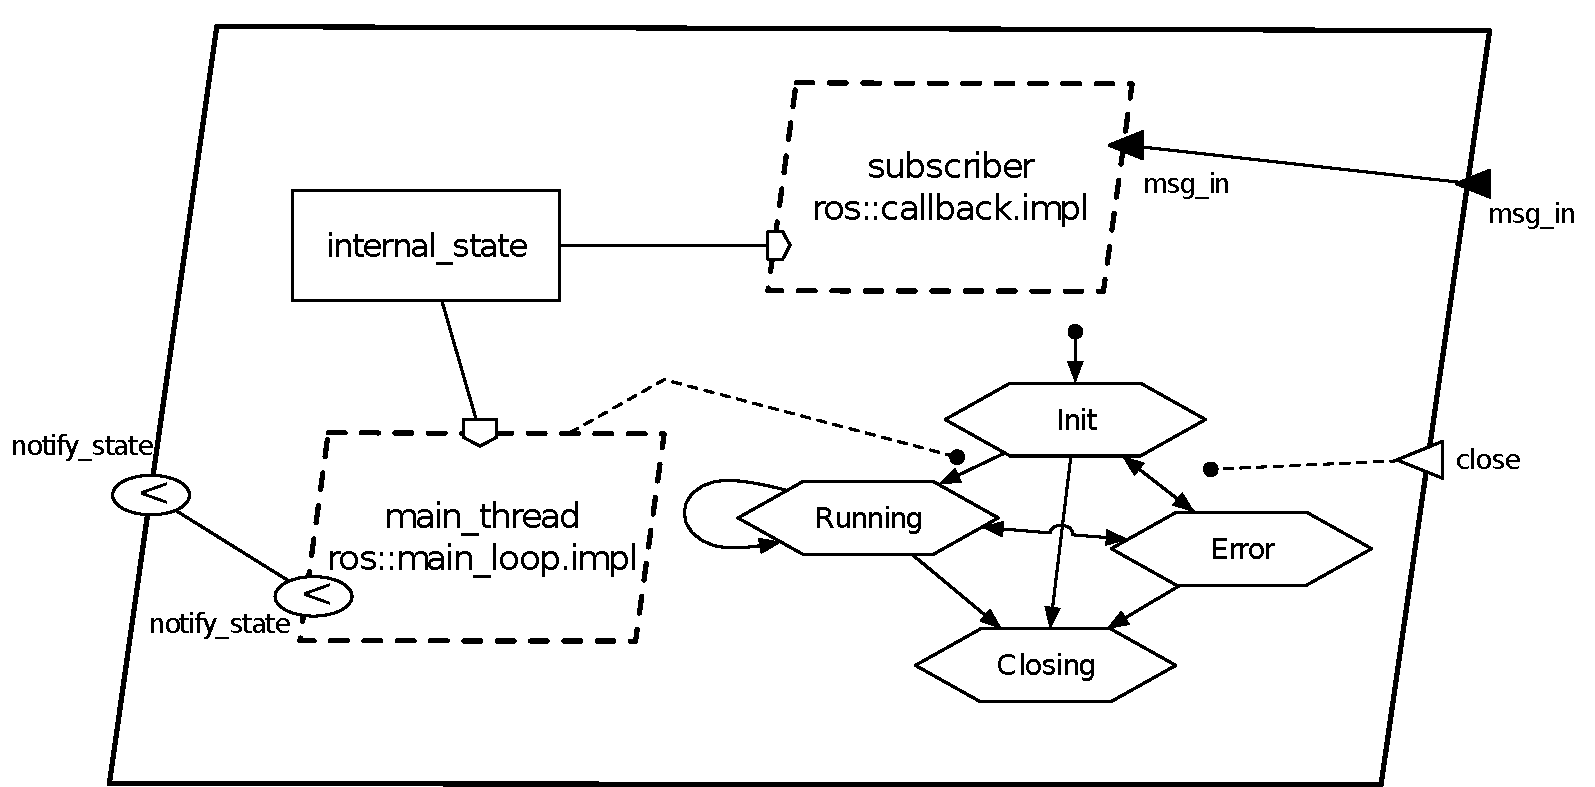
\includegraphics[width=0.9\hsize]{usecase-subscriber}
% \caption{\label{fig:usecase-subscriber}AADL graphical representation of how a \textit{process} (node) including a subscriber \textit{thread} (functionality) looks like.}
% \end{figure}

In Fig.~\ref{fig:usecase-publisher} and Fig.~\ref{fig:usecase-subscriber} are represented, respectively, the publisher and the subscriber models, except for their \textit{properties}. In both cases we have the following \textit{properties}:
\begin{itemize}
\item \textit{Source\_Text} and \textit{Source\_Name}: the first identifies the file where the application specific code will be placed, while the second represents the name of the function that will be called. In the publisher case, this function will return the message to be sent, while, for the subscriber, it will have as input the received message to be processed.
\item \textit{topic\_properties::Default\_Name}: it is the topic name placeholder in order to generate correctly the node. It can be different for the publisher and the subscriber, since the binding between them is done at system’s connections level and it is represent as a \textit{remap} in the ROS launch file.
\end{itemize}

Moreover, the publisher has a specific property, called \textit{Period}, where the frequency of the publisher is defined. The subscriber also has its own specific property called \textit{Queue\_size}, representing the maximum size of the subscriber message buffer.

Models in Fig.~\ref{fig:usecase-publisher} and Fig.~\ref{fig:usecase-subscriber} have the mandatory main thread implementation; it is important to see that the two threads inside the process, namely \textit{main\_thread} and \textit{publisher} or \textit{subscriber}, need to have their ports connected to the process’ ports, thus, at \textit{process} level, we have \textit{connections} and \textit{features} definitions.

In addition, the two figures show the common base model under each node. As stated in in~\cite{Bardaro2017}, the model of the base node contains a state machine, with four different states: \textit{init}, \textit{running}, \textit{closing} and \textit{error}. In AADL, each transition has to be triggered by an event; an event data port on the process models any external signal to force the shutdown of the node (i.e. SIGINT signal) and various ports on the main thread trigger the transition from a state to another. The current node state is saved \textit{data} element called \textit{internal\_state}. For each existing element of the model (i.e. threads, subprograms, connections, ports, etc.) it is possible to define in which state they are active, and this defines a specific workflow and a strict initialization procedure of the node.

In Listing~\ref{snippet:aadl_pub_sub_publisher} we present the code only for the publisher, but extending the same concepts can be easily extended the subscriber case:

\begin{lstlisting}[frame=tb,caption={AADL model for a simple process (node) implementing a publisher feature},label=snippet:aadl_pub_sub_publisher]
process talker extends ros::node
	features
 		msg_out: out data port custom_msgs::Complex;
end talker;

process implementation talker.impl extends ros::node.impl
 	subcomponents
 		publisher: thread ros::publisher.impl (message => data custom_msgs::Complex);
 	connections
 		chatter: port publisher.msg -> msg_out;
 	properties
 		Source_Text => ("Publisher.h") applies to publisher.function;
 		Source_Name => "publisher_function" applies to publisher.function;
 		topic_properties::Default_Name => "/out_topic" applies to msg_out;
 		Period => 10 ms applies to publisher;
 end talker.impl;
 \end{lstlisting}

The above example includes all the already cited components, as well as the thread output port, connected to the process port and the associated properties. It may be worth taking a closer look at how the datatype of the exchanged message is actually defined: the type is associated to the process output port and specified as a prototype of the thread. This ensures the thread type to match the process-level type.
In our example, the message is of \textit{Complex} type defined inside the package \textit{custom\_msgs}. Its definition is shown in Listing~\ref{lst:aadl_custom_msgs}. However, the actual implementation of said definition is enclosed in the \textit{``custom\_msg.asn''} linked file, in ASN.1 language.

\begin{lstlisting}[frame=tb,caption={AADL representation of a custom message},label=lst:aadl_custom_msgs]
data Complex
 	properties
 		Source_Text => ("custom_msg.asn");
end Complex;
\end{lstlisting}


Based on this model, the ROS packages generated by our toolchain have the following structure:
% \begin{itemize}

% \item[] 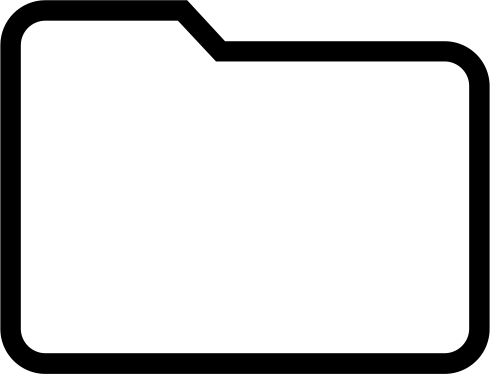
\includegraphics[width=0.3cm]{folder.png} pubsub
% \begin{itemize}
% \item[] 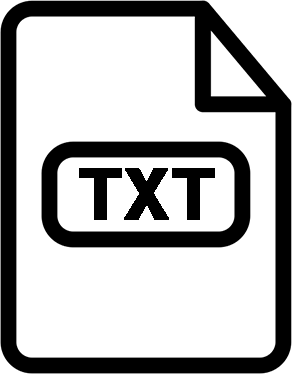
\includegraphics[width=0.3cm]{file_txt.png} CMakeLists.txt

% \item[] 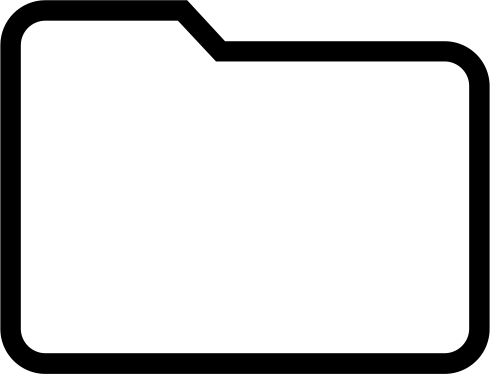
\includegraphics[width=0.3cm]{folder.png} include
% \begin{itemize}
% \item[] 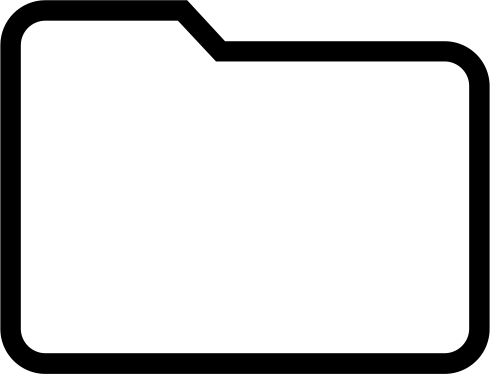
\includegraphics[width=0.3cm]{folder.png} pubsub
% \begin{itemize}
% \item[] 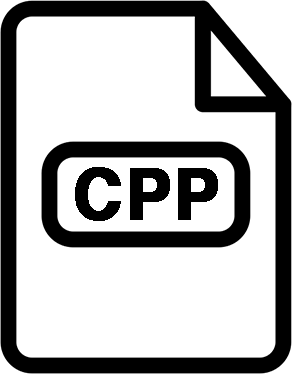
\includegraphics[width=0.3cm]{file_cpp.png} Publisher.h
% \item[] 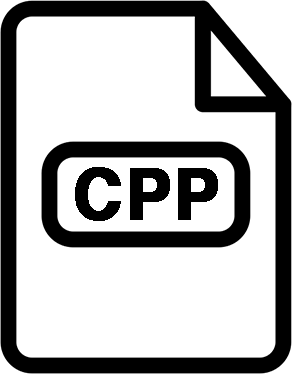
\includegraphics[width=0.3cm]{file_cpp.png} Subscriber.h
% \end{itemize}
% \end{itemize}

% \item[] 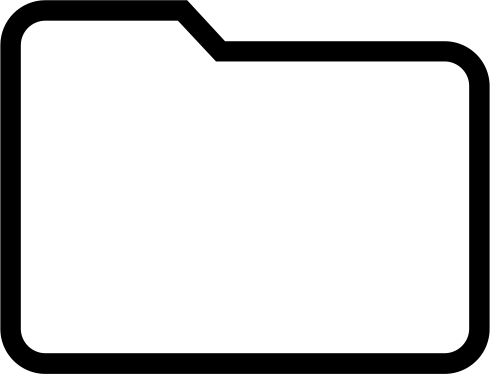
\includegraphics[width=0.3cm]{folder.png} launch
% \begin{itemize}
% \item[] 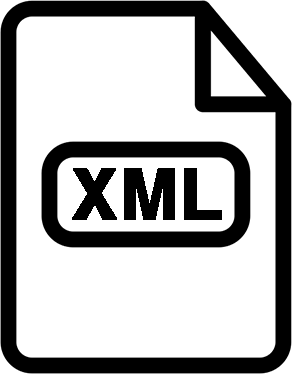
\includegraphics[width=0.3cm]{file_xml.png} container.impl.launch
% \end{itemize}

% \item[] 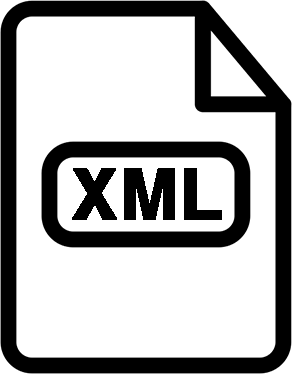
\includegraphics[width=0.3cm]{file_xml.png} package.xml

% \item[] 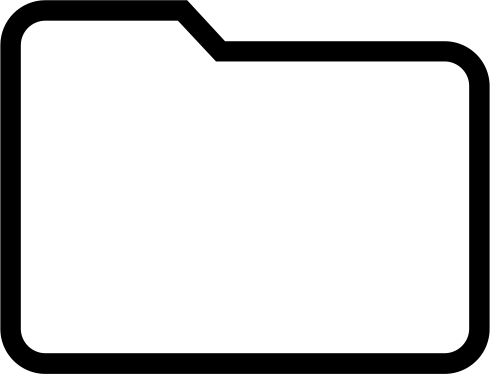
\includegraphics[width=0.3cm]{folder.png} src
% \begin{itemize}
% \item[] 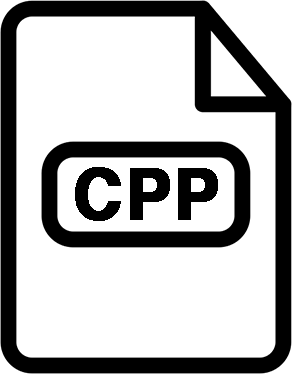
\includegraphics[width=0.3cm]{file_cpp.png} Publisher.cpp
% \item[] 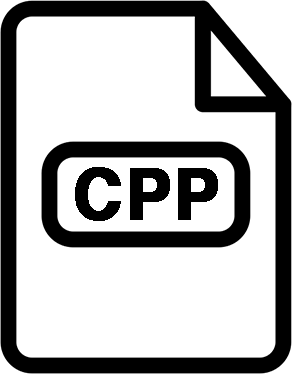
\includegraphics[width=0.3cm]{file_cpp.png} Subscriber.cpp
% \end{itemize}

% \end{itemize}

% \item[] 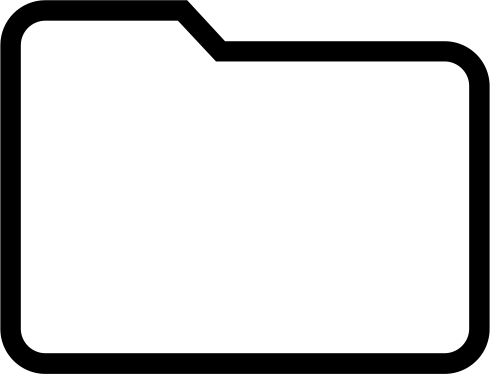
\includegraphics[width=0.3cm]{folder.png} custom\_msgs
% \begin{itemize}
% \item[] 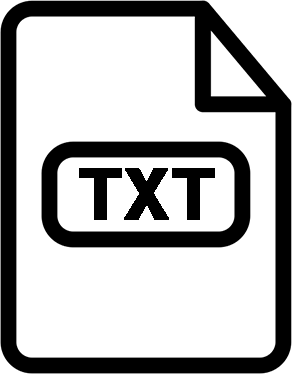
\includegraphics[width=0.3cm]{file_txt.png} CMakeLists.txt

% \item[] 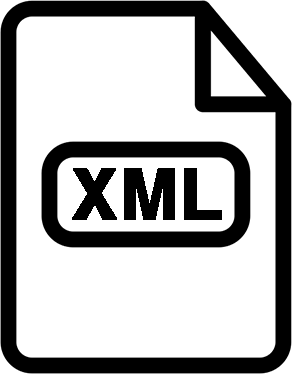
\includegraphics[width=0.3cm]{file_xml.png} package.xml

% \item[] 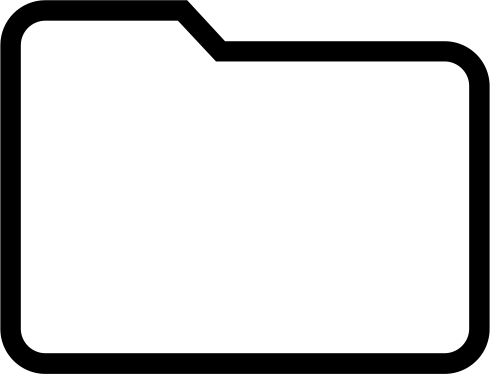
\includegraphics[width=0.3cm]{folder.png} msg
% \begin{itemize}
% \item[] 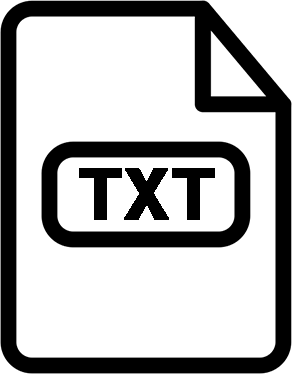
\includegraphics[width=0.3cm]{file_txt.png} Complex.msg
% \end{itemize}

% \end{itemize}
% \end{itemize}

\textit{Publisher.h} and \textit{subscriber.h} can be used as a guideline to implement the application-specific interface. The provided files, already import all the necessary libraries. Further, it is also important to note that decoupling these files from the rest of the ROS nodes, allows developers to test the implemented functions without launching the whole ROS environment at each iteration. This feature 
% simplifies both the developing and testing phases significantly, reducing the computational complexity of the underlying code.


%TODO update this figure to include the GSM
\begin{figure}[t]
\centering
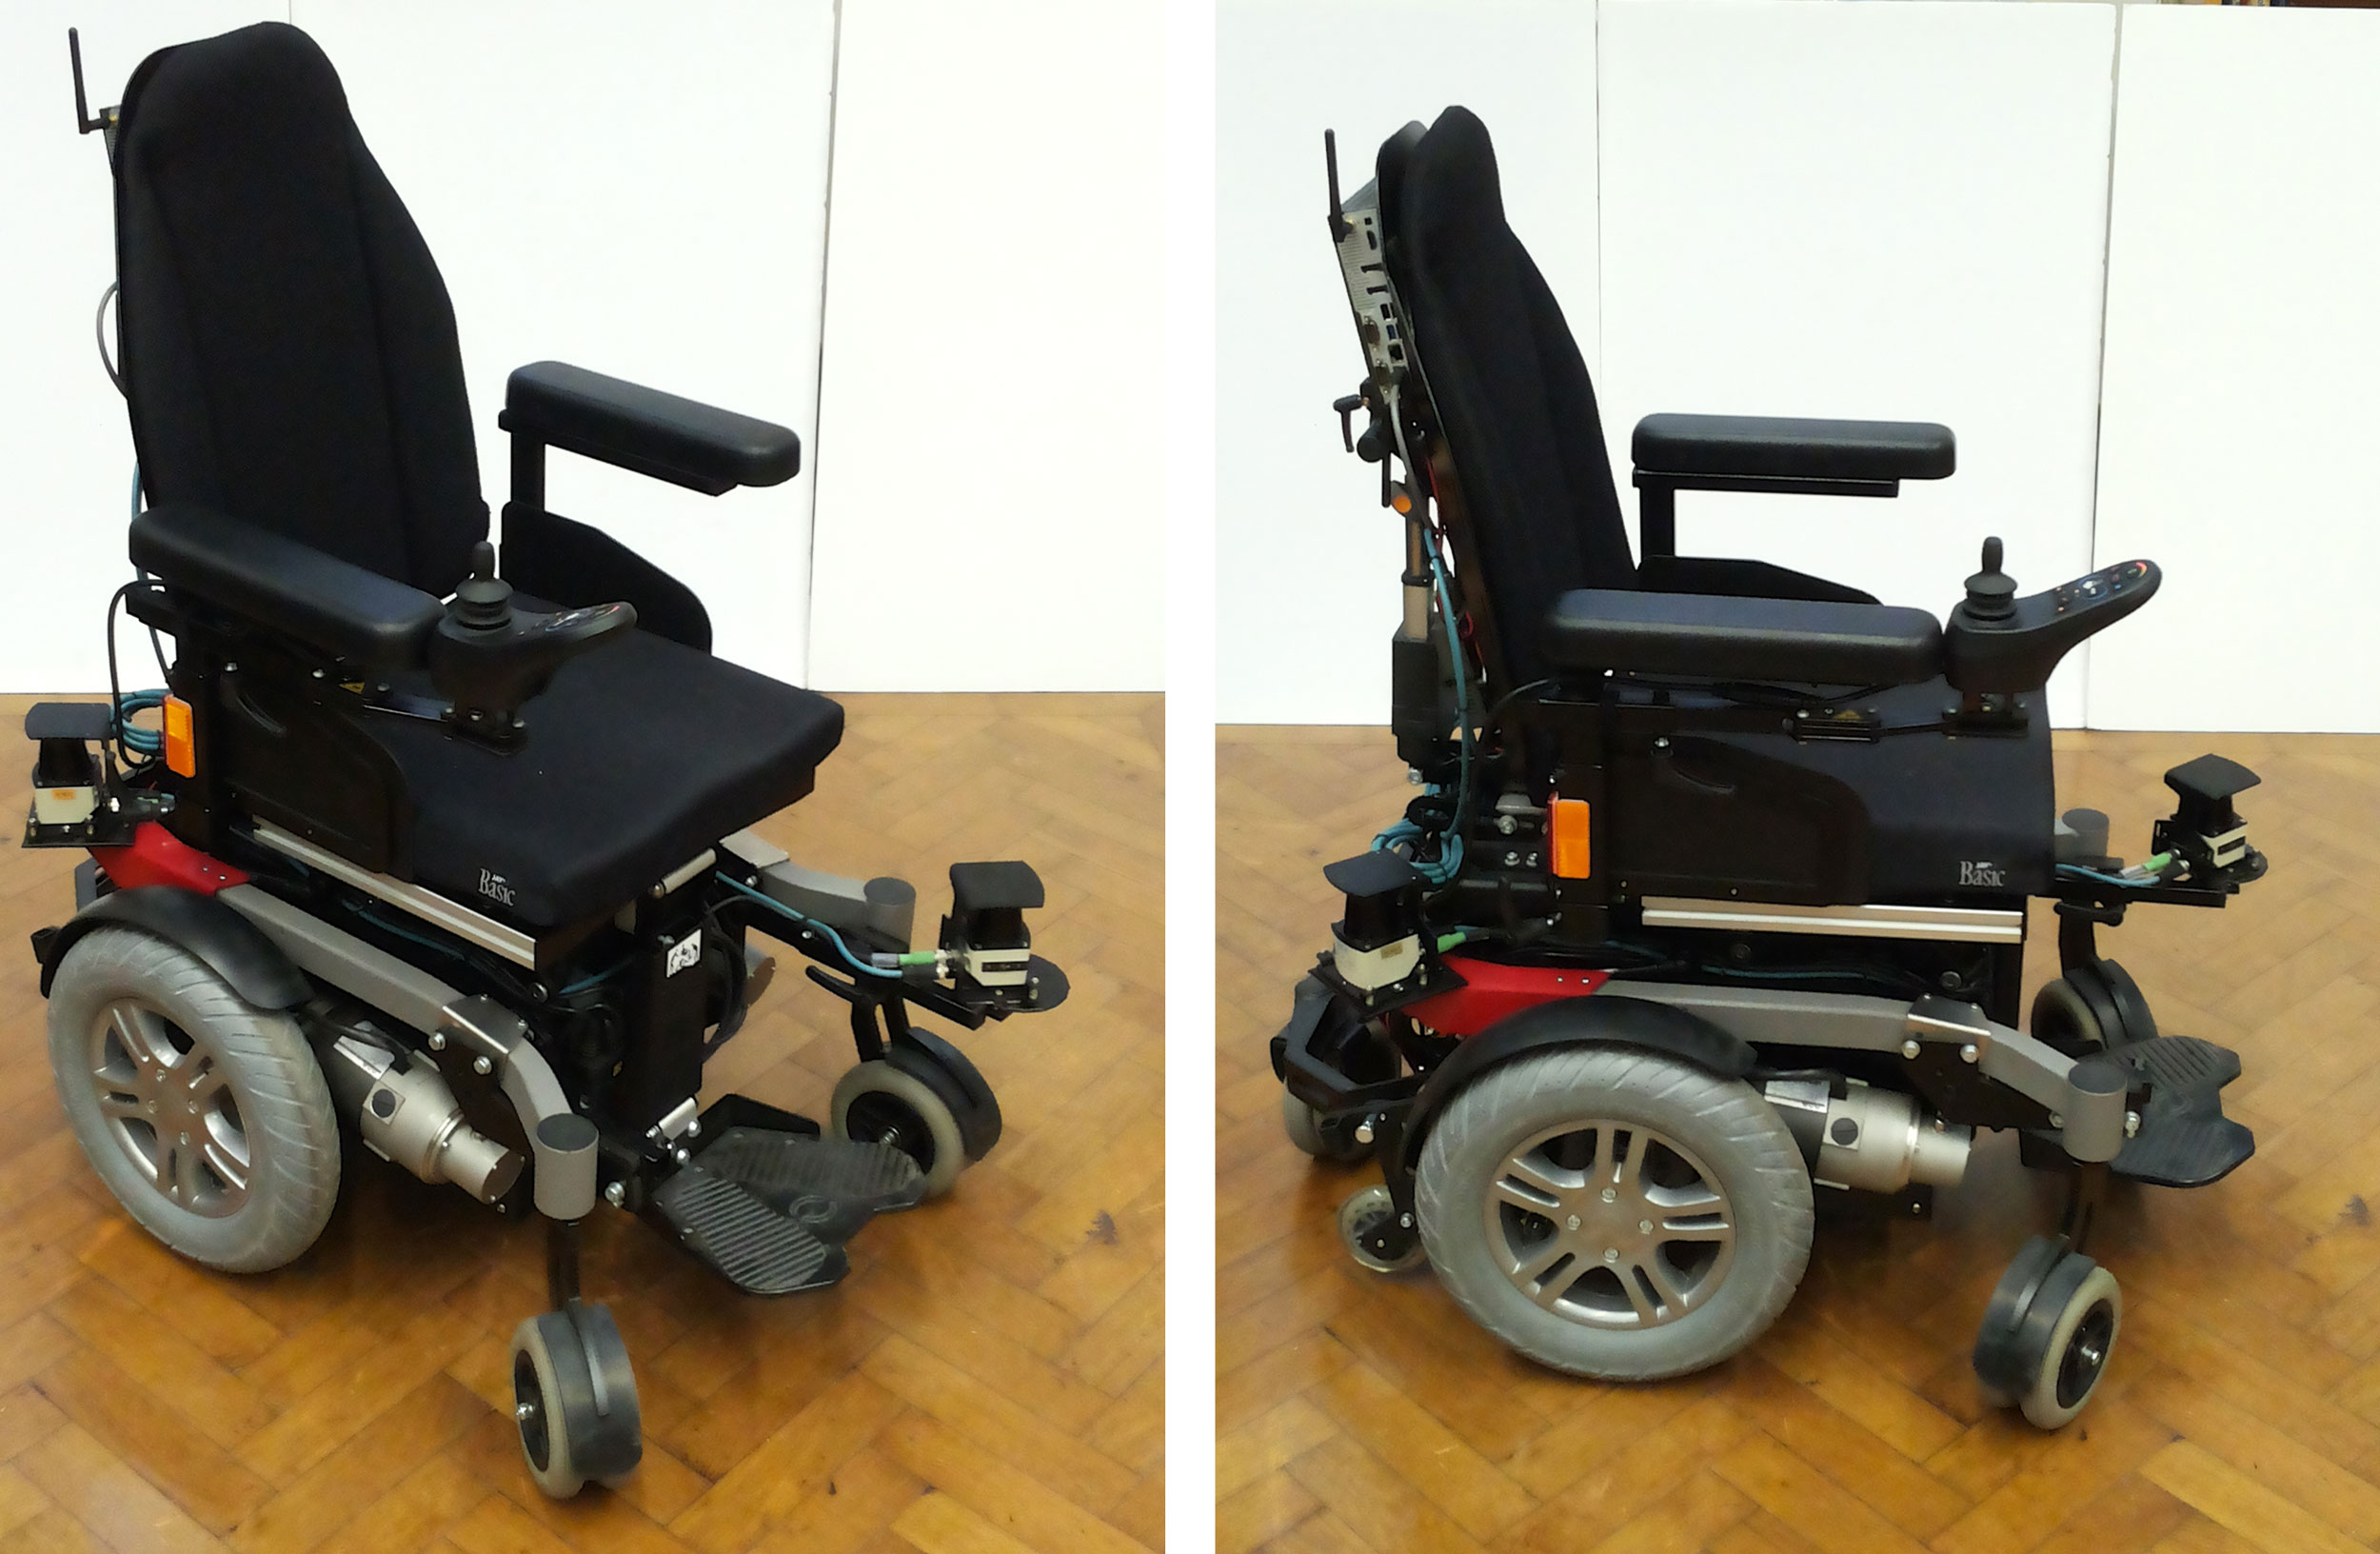
\includegraphics[width=0.95\textwidth]{gfx/pmk/pmk_plat}
\caption{TODO}
\label{fig:pmk}
\end{figure}


\section{The PMK use case}
\label{sec:pmk}
In this section we give a detailed description of a test use case where a model-based approach has been used to replicate and reimplement an existing architecture developed with traditional techniques. We decided to start from an already implemented and fully functional system, to show that is possible to achieve the same level of functionalities of the original application with a model-based design combined with automatic programming.

The target robot is an electric wheelchair modified to be controlled with a computer, and equipped with various sensors to achieve levels of autonomy and teleoperation. The wheelchair used as the starting platform is a commercial model (\textit{Twist T4 2x2}) produced by Degonda Rehab SA; it is suitable for both indoor and outdoor usage and it has high manoeuvrability thanks to the two-wheeled dynamics. The conversion from traditional electric wheelchair to autonomous robotic platform is achieved using the Personal Mobility Kit (PMK), which consists in four elements.
\begin{itemize}
\item Encoders connected to the electric motors controlling the wheels, they provide odometry information.
\item Two \textit{Sick TiM 561} laser scanner distance sensors, they provide a 360-degrees coverage around the wheelchair. They are used to map the environment, assist in the localisation of the robot and detect unexpected obstacles.
\item \textit{Shuttle DS81L}, an high-performance slim PC specifically designed for automotive and robotics applications. It is the on-board computer of the robot, it runs ROS and all the application code.
\item The software components necessary to achieve the assisted and autonomous functionalities.
\end{itemize}
The PMK is designed to be an add-on that is possible to mount over any existing electric wheelchair to convert it into an autonomous or semi-autonomous platform. Thus, of the architecture we will present, the only platform specific part is the interface used to interface with on-board electronics, everything else is a modular design that can be adapted to multiple physical platforms.

A commercial electric wheelchair supports manual control through a joystick placed on one of the armrest. While this is suitable for most of users, there are cases of severe disabilities where the patients can only partially or cannot operate the joystick. The objective of PMK is to extend the functionalities of an electric wheelchair to provide assisted and autonomous control. In particular, the implemented software supports four different drive modes.

\paragraph{Manual with PMK off} This is the native configuration of the wheelchair, the user controls the movements directly with the on-board joystick. It is important to maintain the original operational mode even after the modification introduced by the PMK, the electric wheelchair should remain completely functional and operative even if an hardware or software malfunction causes the PMK to stop working. This act as a fallback emergency configuration.
\paragraph{Manual with PMK on} In this configuration the PMK is active, but the user is still completely in control of the wheelchair. When mediated by the software system, the robotic platform can be controlled remotely by using a wireless joypad or directly with the on-board joystick, a priority system ensures that the input from the joystick always has precedence over teleoperation. This is the neutral configuration of PMK, when the system is active, but not performing any action. This mode is particularly useful during the set up phases of the autonomous wheelchair (\eg, environment mapping).
\paragraph{Assisted} In this mode the PMK is enabled and actively meditates the commands coming from any input device. The aim of this configuration is to help the user operate the wheelchair by avoiding obstacles. Set-points sent from the wireless joypad or on-board joystick are processed and, if necessary, modified to avoid obstacle perceived by the two on-board laser scanners. As for the previous mode, the commands coming from the joystick have the priority over the wireless joypad.
\paragraph{Autonomous} Here the wheelchair is fully autonomous, the PMK is in charge of controlling the movements. The user can request a specific goal (\eg, ``take me to the kitchen''), then the robotic platform will automatically reach the destination avoiding any obstacle along the way. For safety reasons, it is always possible to override the commands sent by the PMK in autonomous mode using the on-board joystick.

\medskip
These are all the main functionalities of the electric wheelchair when equipped with the Personal Mobility Kit. Our aim is to create a system designed and developed using a model-based approach combined with automatic programming that exploits all the problem-related implementations already created for the original architecture and combine them with automatically generated ROS nodes, while maintaining the same functionalities.

\begin{landscape}
	\begin{figure}[t]
	\centering
	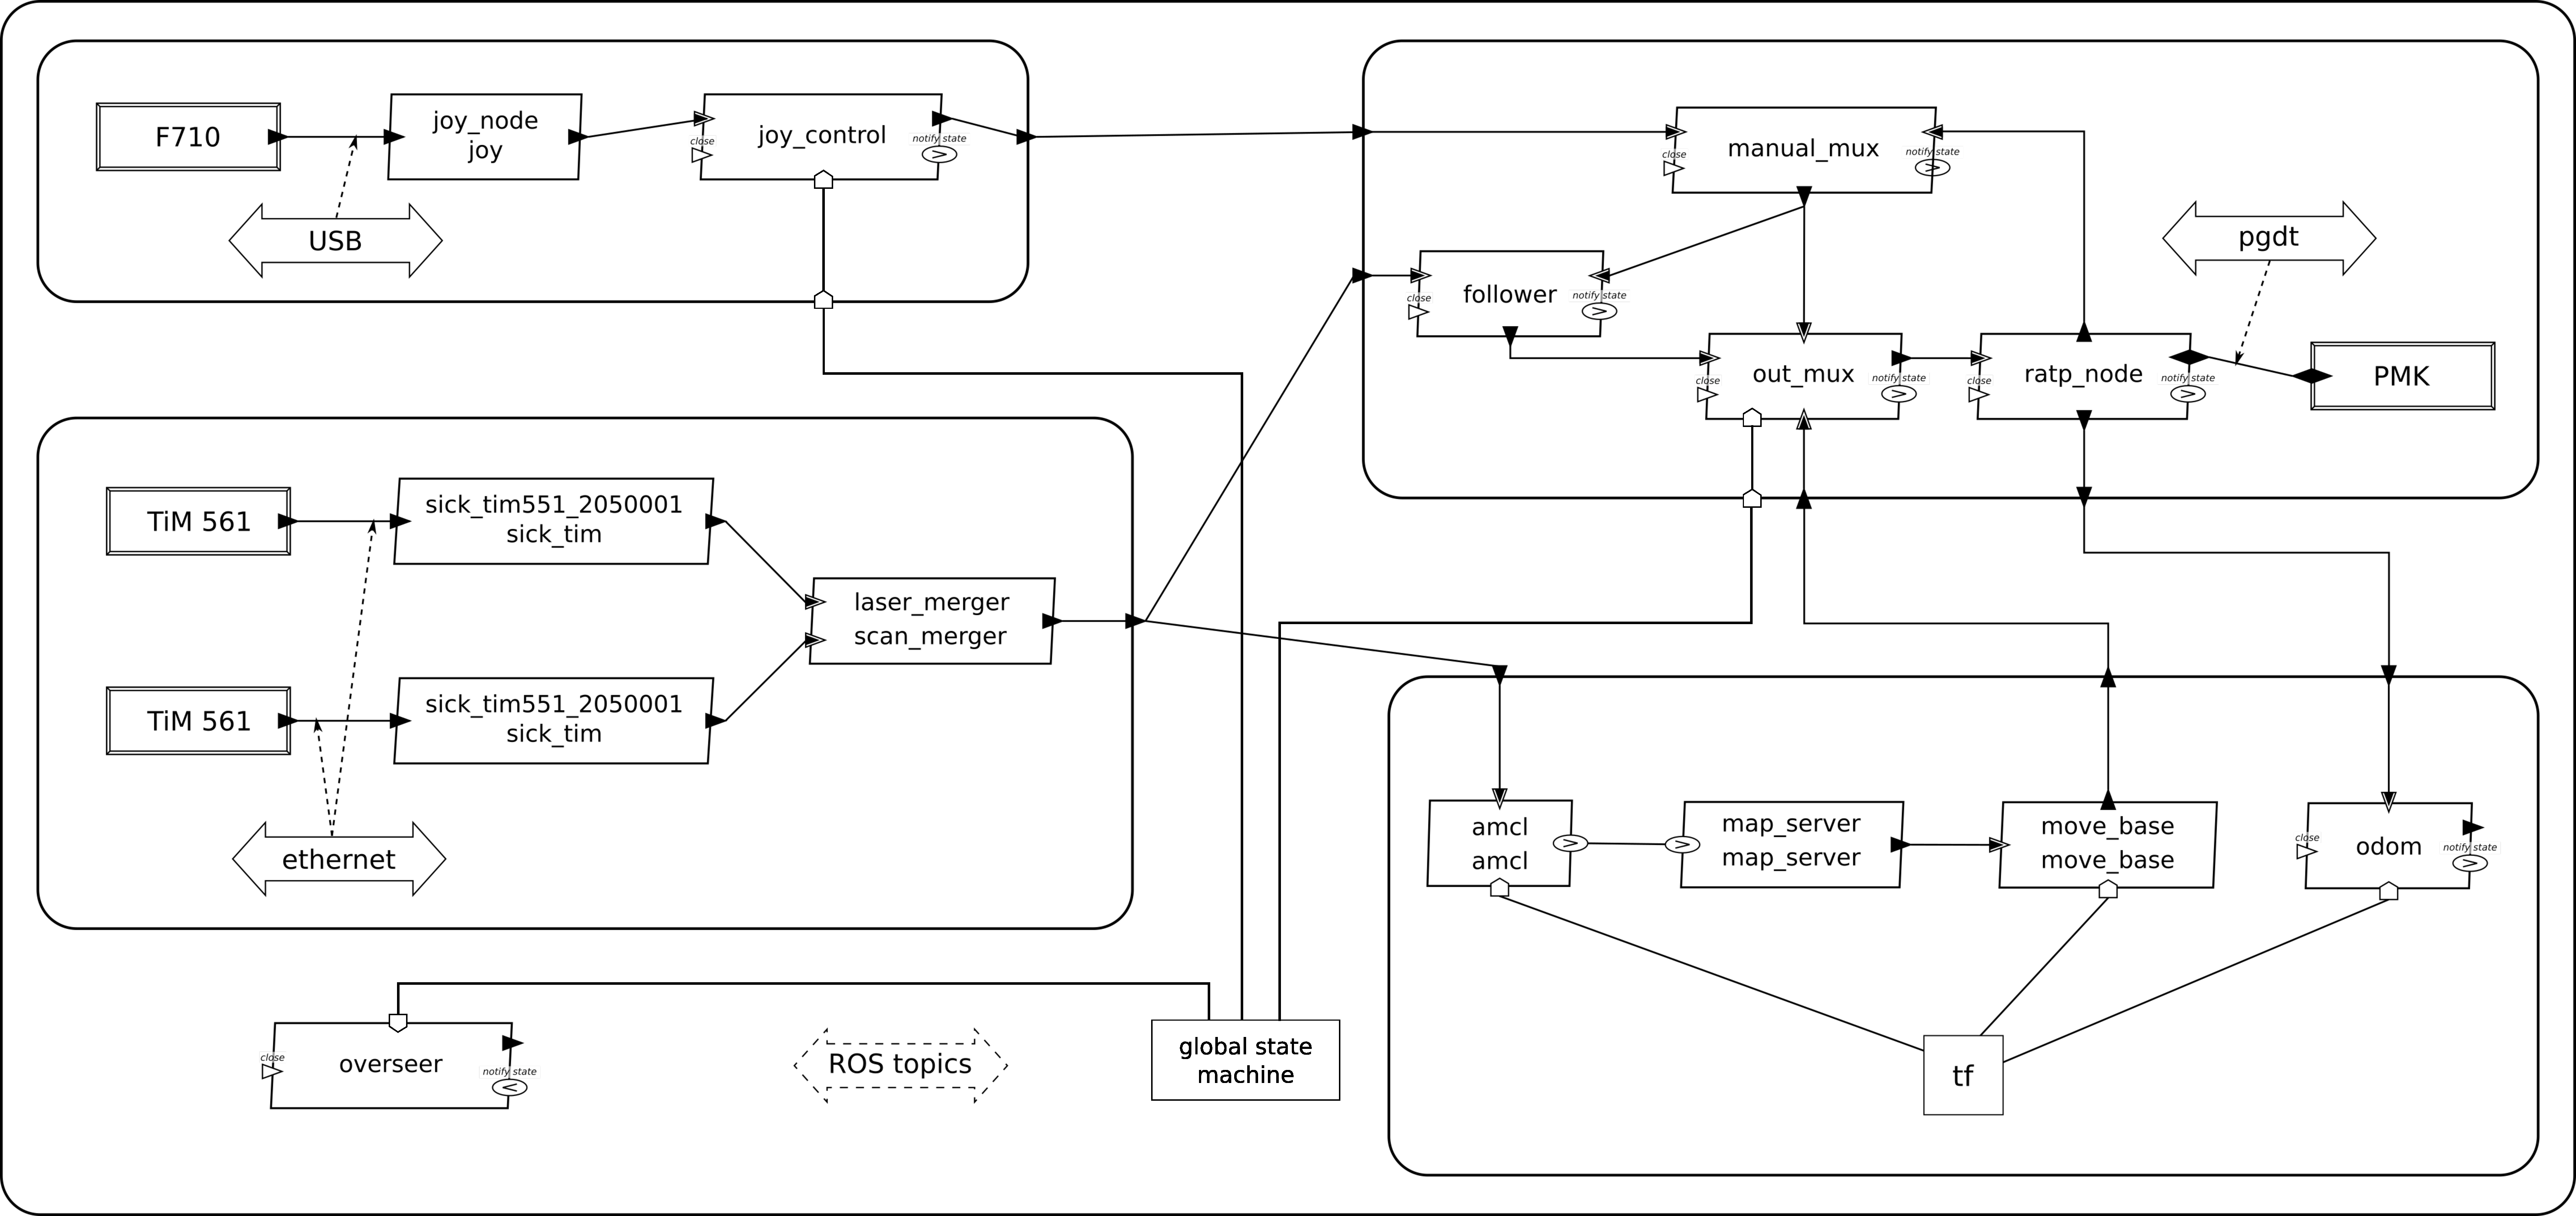
\includegraphics[width=0.95\textheight]{gfx/pmk/model}
	\caption{TODO}
	\label{fig:pmk-model}
	\end{figure}
\end{landscape}


\subsection{Model}
\label{sec:pmk-model}
The first step of the design of an architecture is to create the model. We did so by following the definitions and meta-models introduced in Chapter~\ref{ch:Modelling}. Figure~\ref{fig:pmk-model} shows a graphical representation of the complete model of the architecture of the robotic wheelchair. To organise and generalise the architecture we exploited the nesting capability of AADL by creating a hierarchical structure of system of systems. Each subsystem capture a specific functionality of the robot, and they are meant to be modular parts of the design that can be replaced when necessary. For example, going from laser scanner to cameras, or replacing the navigation system based on \textit{move\_base} with a custom one, or using a different electric wheelchair as platform.

\paragraph{Teleoperation} Similarly to the example presented in Section~\ref{sec:ros-arch}, this subsystem captures all the hardware and software components necessary to implement teleoperation. This specific models includes an AADL device modelling the wireless joypad used to control the wheelchair, a Logitech Gamepad F710. Directly connected to it, the device driver, the existing ROS node \textit{joy\_node} from the package \textit{joy}; it reads the input from the joypad and converts it to ROS messages. The connection between the device and the driver is bound to an AADL bus modelling the physical USB interface between the joypad and the computer. The last software component in the subsystem is a node specifically designed for this application, \textit{joy\_control} is in charge of converting the messages coming from the device driver to velocity set-points to directly control the wheelchair (\ie, from \textit{Joy} to \textit{Twist} messages). Additionally, this node controls the global state machine of the system that selects the current driving mode (\ie, one of the four presented in Section~\ref{sec:pmk}), given the criticality of this communication it does not happen through ROS topics or services, but by accessing directly a shared memory area. This behaviour is captured in the model using a require data access port on the process modelling \textit{joy\_control}. On its frontier, the system exposes an outgoing port associated with the velocity command to relay the set-points generated by the teleoperation subsystem to the rest of the architecture; moreover it has a data access to bridge the connection coming from the driving mode selection node (\ie, \textit{joy\_control}) to the shared memory area hosting the global state machine. Encapsulating the model in a system increases the modularity of the design, since it defines exactly the expected interfaces of the subsystem and makes it replaceable with a similar configuration (\eg, a different physical input) without altering the entire architecture.

\paragraph{Sensing} For the navigation and obstacle avoidance to work correctly, they need a single measurement from the laser rangefinder. Since the robotic platform is equipped with two sensors, the aim of the sensing subsystem is to unify their measurements in a single output; for this reason only one outgoing port is present on the system frontier representing the merged scan topic. Here there is a clear example on how multiple instances of same element can coexist as subcomponents. There are two occurrences of the same AADL device modelling the physical sensors mounted on the wheelchair, consequentially, the device driver component is duplicated too. As for the teleoperation subsystem, the connection between each laser scanner and the corresponding driver is bound to a model of a physical bus; but since the communication goes through an Ethernet connection it is a different component. All the connections converge in a single node in charge of merging the measurements coming from each laser rangefinder, that are then relayed outside the subsystem through the output port present on the frontier. In this system there is no custom node, since all of them come from existing packages or legacy implementations.

\paragraph{Navigation} This subsystem mostly contains legacy nodes from ROS Navigation. A node implementing adaptive Monte Carlo localisation to estimate the position of the robot in a known environment (\textit{amcl}), a node to store and share the current map of the environment (\textit{map\_server}), and the main navigation node (\textit{move\_base}) implementing global planning on the known map and local planning on the map generated in real time. To work, ROS Navigation requires laser measurements and odometry information, the former comes from the sensing subsystem, while the latter is generated by the custom \textit{odom} node included in the navigation subsystem; it receives the current speed from the wheelchair and uses it to estimate the position of the platform. The odometry node supports two types of output, as visible from the features of the AADL process, an \textit{Odometry} message, published on a topic and modelled using an output port, and shared using \textit{tf}, modelled thorough a data access directly connected to the data component representing the centralised collection of all the reference frames. Since it is the backbone of ROS Navigation, and it is used only by nodes in this subsystem, it was reasonable to model the data component representing \textit{tf} here. Differently from the two previous subsystems (\ie, teleoperation and sensing), here there is no need to model any physical bus since this is a pure software system. The frontier of the navigation subsystem is more complex, since it has an input port for the laser measurements, another input port for the speed of the wheelchair and  an output port for the set-point generated by \textit{move\_base}. Abstracting the structure and interface of the navigation subsystem is particularly important since it is the part of the architecture that is more subject to changes, it is common to use the same platform to test different algorithms and architectural solutions for navigation.

\paragraph{Platform} All the hardware and software components related to the physical platform are contained in this subsystem, since they are all platform-related, each node is a custom design created specifically for this architecture. There are two hardware components: a device to model the interface between the architecture and the on-board electronics manufactured by Penny\&Giles Drive Technologies Ltd. (PGDT), and the bus representing the special hardware connection used to exchange wheelchair-specific messages. This bus and the corresponding custom device driver (\textit{ratp\_node}) act as a bridge between platform-specific data streams and ROS messages. Given the multiple driving modes of the robot where two manual inputs, potentially mediated by the system and with different priorities, coexists, together with an autonomous mode, the architecture uses a combination of two multiplexers. One is used to select the specific manual input (\ie, \textit{manual\_mux}), while the other (\ie, \textit{out\_mux}) differentiate between the different driving modes (\ie, manual, assisted and autonomous). The two multiplexers have different behaviours, \textit{manual\_mux} is based on priorities, the input coming from the the on-board joystick will always override the wireless joypad, while \textit{out\_mux} changes the output depending on the current mode of the system, for this reason this component has a data access connected to the shared memory area hosting the global state machine. Finally, the last component is a node implementing local obstacle avoidance for assisted driving. Even with its peculiar configuration, the whole subsystem is designed with a general frontier, it exposes two inbound ports for the velocity commands (\ie, joypad and autonomous set-points) and one for scan messages (\ie, measurements for obstacle avoidance). The output port relays the current velocity of the wheelchair from the custom device driver node to the navigation subsystem. Additionally, as for the teleoperation subsystem, the platform system has a data access on its frontier to connect to the global state machine. By encapsulating the platform in a system, it is possible to replace it with a different wheelchair, or even with a completely different robotic platform.

\begin{figure}[t]
\centering
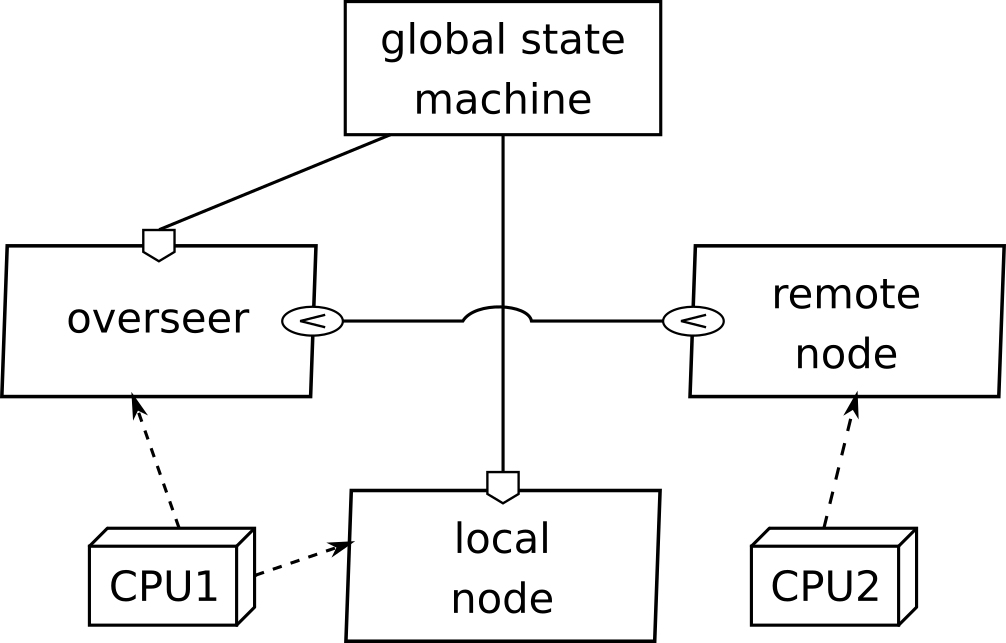
\includegraphics[width=0.7\textwidth]{gfx/pmk/overseer}
\caption{TODO}
\label{fig:pmk-gsm}
\end{figure}

\paragraph{Main system} To increase clarity and use the model to evoke the modularity of the architecture, we modelled it with different subsystems. However, in AADL it is necessary to define a root system to encapsulate everything, moreover, some part of the architecture are too general to be fitted in a specific subsystem. For this architecture, three components fall in this category: the \textit{ROS communication} virtual bus, the \textit{overseer} node and the global state machine. In the same way as physical buses are used in the teleoperation and platform subsystems, the \textit{ROS communication} virtual bus is necessary to identify which connections model ROS communication protocols (\ie, topics or services), this is done by binding them to it. As originally introduced in Section~\ref{sec:ros-in-aadl} and, later, detailed in Section~\ref{sec:ros-node}, the engineered nodes are designed with a strict life cycle, and they natively support a notification system to monitor the evolution of their state. The \textit{overseer} node is in charge of collecting all the notification coming from the custom nodes, moreover it has a list of all the critical nodes (\ie, nodes that are subject to a liveness check) and trigger a transition on the global state machine if one of them stops working. The last element is the data component representing the shared memory area containing the global state machine. In the implementation, the global state machine is instantiated by the \textit{overseer}, while all the nodes in the architecture can read or modify the current state by accessing the shared memory directly, it is also possible to interact with the global state machine through a ROS service interface mediated by the \textit{overseer} (see Figure~\ref{fig:pmk-gsm}). The different approach used can be encoded in the model (\ie, connected through a data access or a subprogram call) however, in the implementation, it is determined at deployment time. In practice if the node runs on the same physical machine of the global state machine, then a shared memory approach is used, otherwise the interaction happens using ROS. 

\subsection{Automatic code generation}
In the previous section, we gave an overview of the model of the architecture by describing in details the subsystems and which functionalities they evoke. While the graphical representation of Figure~\ref{fig:pmk-model} provides a general understanding of the topology of the architecture and gives some insights on the nature of the components, it does not capture all the details necessary to correctly perform automatic code generation. First of all, nodes belongs to three main categories: already implemented nodes, they are legacy nodes previously developed, they may come from the standard ROS repositories (\eg, \textit{move\_base}) or be part of the original architecture (\eg, \textit{laser\_merger}), custom nodes, they are completely modelled and will be automatically generated (\eg, \textit{odom}), special custom nodes, they are modelled correctly, but they contain unique implementation patterns that are not supported by the code generator (\eg, \textit{ratp\_node}). This last category will be covered in details in Section~\ref{sec:special-node}. 

As discussed in Section~\ref{sec:ros-arch}, managing existing nodes in the architecture model is extremely important, since they are an invaluable resource provided by the ROS community. During the automatic code generation, existing nodes are ignored, since they do not provide any internal implementation but are described only as interfaces, however, they are correctly included in the generation of launch files describing the current configuration of the system. Moreover, connections between components can be specialised using properties to exploit topic remapping and define the runtime name of each topic, included those of already implemented nodes. Currently, the code generator does not support the use of neither ASN.1 nor JSON schema to define the parameters of the legacy nodes, however,  it is possible to use properties to specify a standard ROS YAML file to be automatically included in the launch file as the parameter configuration of a specific node.

To automatically generate custom nodes that are compilation-ready, it is necessary to specify a series of properties. On a basic level, the designer can tune the behaviour of publisher and subscriber by setting the frequency, the queue size or the default name of the topic. Moving to a domain-specific point of view, the developer has to provide the implementations of the nodes; for this reason we decided to base our test use case on an existing architecture to exploit already implemented problem-specific code for the automatic programming phase. To understand how the process works in practice, let us take the example of the \textit{follower} node. Without consider the domain-specific implementation, this component evokes a combination of a \textit{sink} behaviour, the subscriber receiving the messages from the laser rangefinder, and a \textit{filter} behaviour, manual set-points are received, modified according to the scan measurements, eventually modified and published. This configuration is translated to the code generator to two subscribers (\ie, one for the laser and one for the input commands) and a publisher (\ie, the output set-point). Moreover, by parsing the JSON files specified as properties in the component definition, the code generator can create the internal state of the node and set default and initial values for parameters and variables. After generating all the necessary source files, it is possible to include the domain-specific implementation as an external library, defined again in properties of threads and subprograms; this is done by carefully generating all the build files that bind together the auto-generated node skeleton and the manually implemented problem-specific code. When all the file related to the node are fully generated (\ie, core node implementation, internal state, external libraries, and build configurations), it is time to create the launch files. Since the \textit{follower} node is part of the platform subsystem, it will be included in the platform-specific launch file, here the runtime configuration of the node is generated from the JSON files and included, moreover, as for the legacy nodes, the topics name are remapped according to the properties defined on the connections in the model. At this point, the generation of the node is complete and it is ready to be compiled and run.

\begin{figure}[t]
\centering
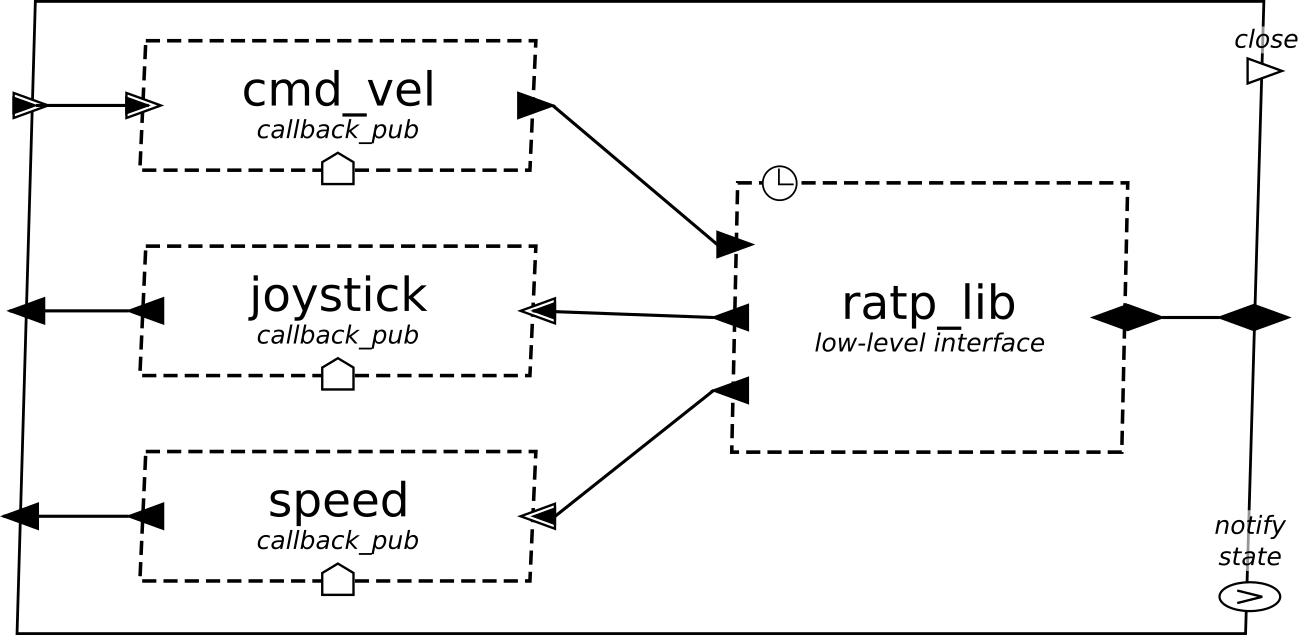
\includegraphics[width=0.95\textwidth]{gfx/pmk/ratp}
\caption{TODO}
\label{fig:pmk-ratp}
\end{figure}

\subsection{Special nodes}
\label{sec:special-node}
Since all the problem-specific logic was already implemented in the original architecture, every element of the new system is generated using the automatic programming approach. There is only one exception: the \textit{ratp\_node}; this node is the device driver connecting the low-level electronics of the wheelchair to the ROS-based architecture. It implements a unique interface between ROS messages and custom data streams defined by the PGDT bus, therefore it is very challenging to automatically generate the source code using an automatic programming approach. Since this node is an hybrid between a ROS-based (\ie, receiving set-points and publishing the current speed and status) and an hardware-specific (\ie, interfacing with the PMK) implementation, we can partially exploit the code generator to define a node skeleton to be refined by the developer. There are two key challenges when using this approach: first, to have a model expressive enough to capture the peculiar design of the component, and second, to generate a node in such a way that the hardware-specific functionalities can be integrated without major modifications.

To tackle the first challenge we can exploit the expressive power provided by AADL. When not extending our base templates (see Section~\ref{sec:template}) used to identify ROS elements,  AADL connections, ports and threads can be used to model any kind of communication protocol or execution flow. Figure~\ref{fig:pmk-ratp} shows a simplified (recurring elements of the base ROS node are omitted) graphical representation of the model of the \textit{ratp\_node}. It is possible to use a periodic AADL thread together with a bidirectional port on its frontier to model the communication between the component and the low-level hardware. Additional ports model the exchange from a problem-specific implementation to the ROS communication protocols.  The \textit{ratp\_lib} thread produces two outputs that are converted to ROS messages: one is the current set-point provided by the on-board joystick, and the other is the current speed of the wheelchair. Moreover, it receives one input from the rest of the system that is then converted to a format compatible with the low-level hardware: the set-point of the current active input. These port on the frontier of the low-level communication thread are connected using internal connections to the corresponding threads modelling the publishers and subscribers. However, there is a significant distinction between this model and how ROS thread are usually modelled. Threads behaving as subscribers are not triggered by a message coming from outside the component, but directly by the \textit{ratp\_lib} thread, moreover, the publisher thread output does not relay its message to the rest of the architecture, but the output port is connected directly to the low-level communication thread.

The second challenge is implicitly solved by the design of the engineered node and how unknown subcomponents are managed by the code generator.  As explained in Section~\ref{sec:xml-cpp}, the code generator parses a process model and implements it as a ROS node, only if it extends the base ROS node model, moreover, of all the threads defined as subcomponents those that do not extend one of the predefined functionalities (\ie, publisher, subscriber, subscriber with publisher or service) are ignored and not processed by the automatic programming system. In the case of the \textit{ratp\_node} it means that the code generator recognises the component as a ROS node and generates all the basic structure, additionally, the three thread modelled as ROS elements (\ie, \textit{cmd\_vel}, \textit{joystick} and \textit{speed}) but connected to the \textit{ratp\_lib} thread are correctly generated as ROS subscribers or publishers. In summary, given the model presented in Figure~\ref{fig:pmk-ratp}, the resulting generated node extends the engineered node and correctly implements the life cycle, the asynchronous spinner, the encapsulated internal state and the separation between the middleware and the problem-specific code; moreover it contains three publishers and three subscribers. Out of these six ROS functionalities, three are already correctly implemented: the publisher for the current speed and the current command of the on-board joystick, and the subscriber for the external set-point. The other three needs to be converted from a ROS-based design to an implementation compatible with the low-level interface. While this approach may appear as an over-complication, it actually streamlines the work of the developer. The code generator handle automatically all the ROS-related boilerplate, while defining a structure that can be easily exploited; the developer only needs to focus on implementing the thread interfacing with the low-level hardware. In our implementation, we use the already created structure as a reference and replaced the callback structure of ROS with standard bindings. Basically, from the point of view of the node, the interaction still happens through a system of callbacks, however, they are not triggered by ROS, but controlled by the \textit{ratp\_thread}. 

In conclusion, while this node requires a direct intervention of the developer to modify its structure, it is more efficient to model it, generate the code to obtain a partially implemented component and then manually insert some modifications, instead of implementing it from scratch. This is possible because of the modularity and flexibility of the engineered node, and because ROS is still the main element of the component design. While our code generator currently cannot completely and successfully process this type of nodes, this mixed approach (\ie, code generation combined with heavy human intervention) gives us an insight on how future nodes with the same characteristics could be automatically generated.


\begin{landscape}
	\begin{figure}[t]
	\centering
	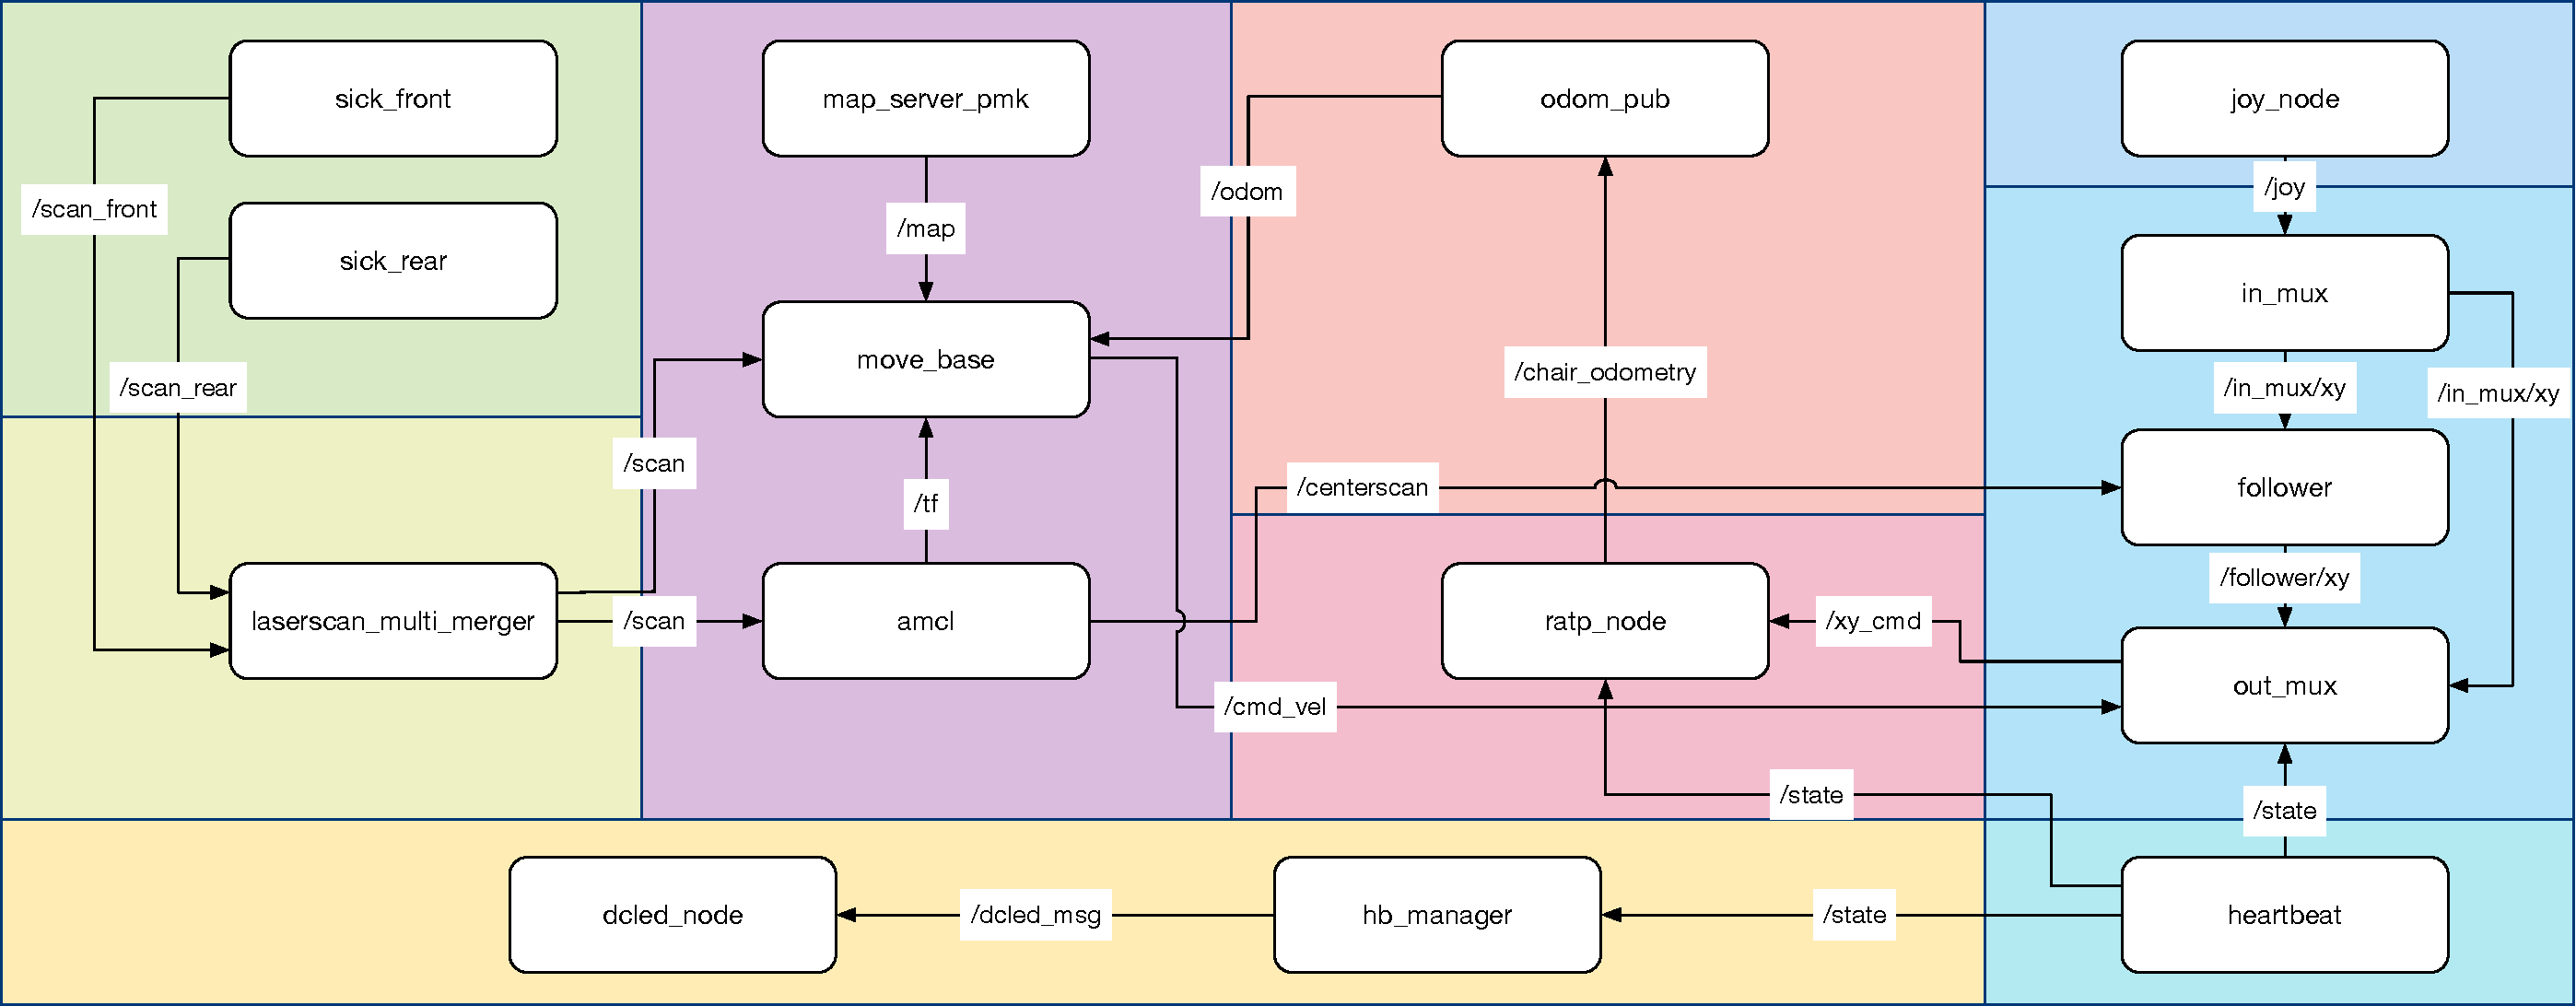
\includegraphics[width=0.95\textheight]{gfx/pmk/softwarearchitecture}
	\caption{TODO}
	\label{fig:pmk-doc}
	\end{figure}
\end{landscape}

\begin{landscape}
	\begin{figure}[t]
	\centering
	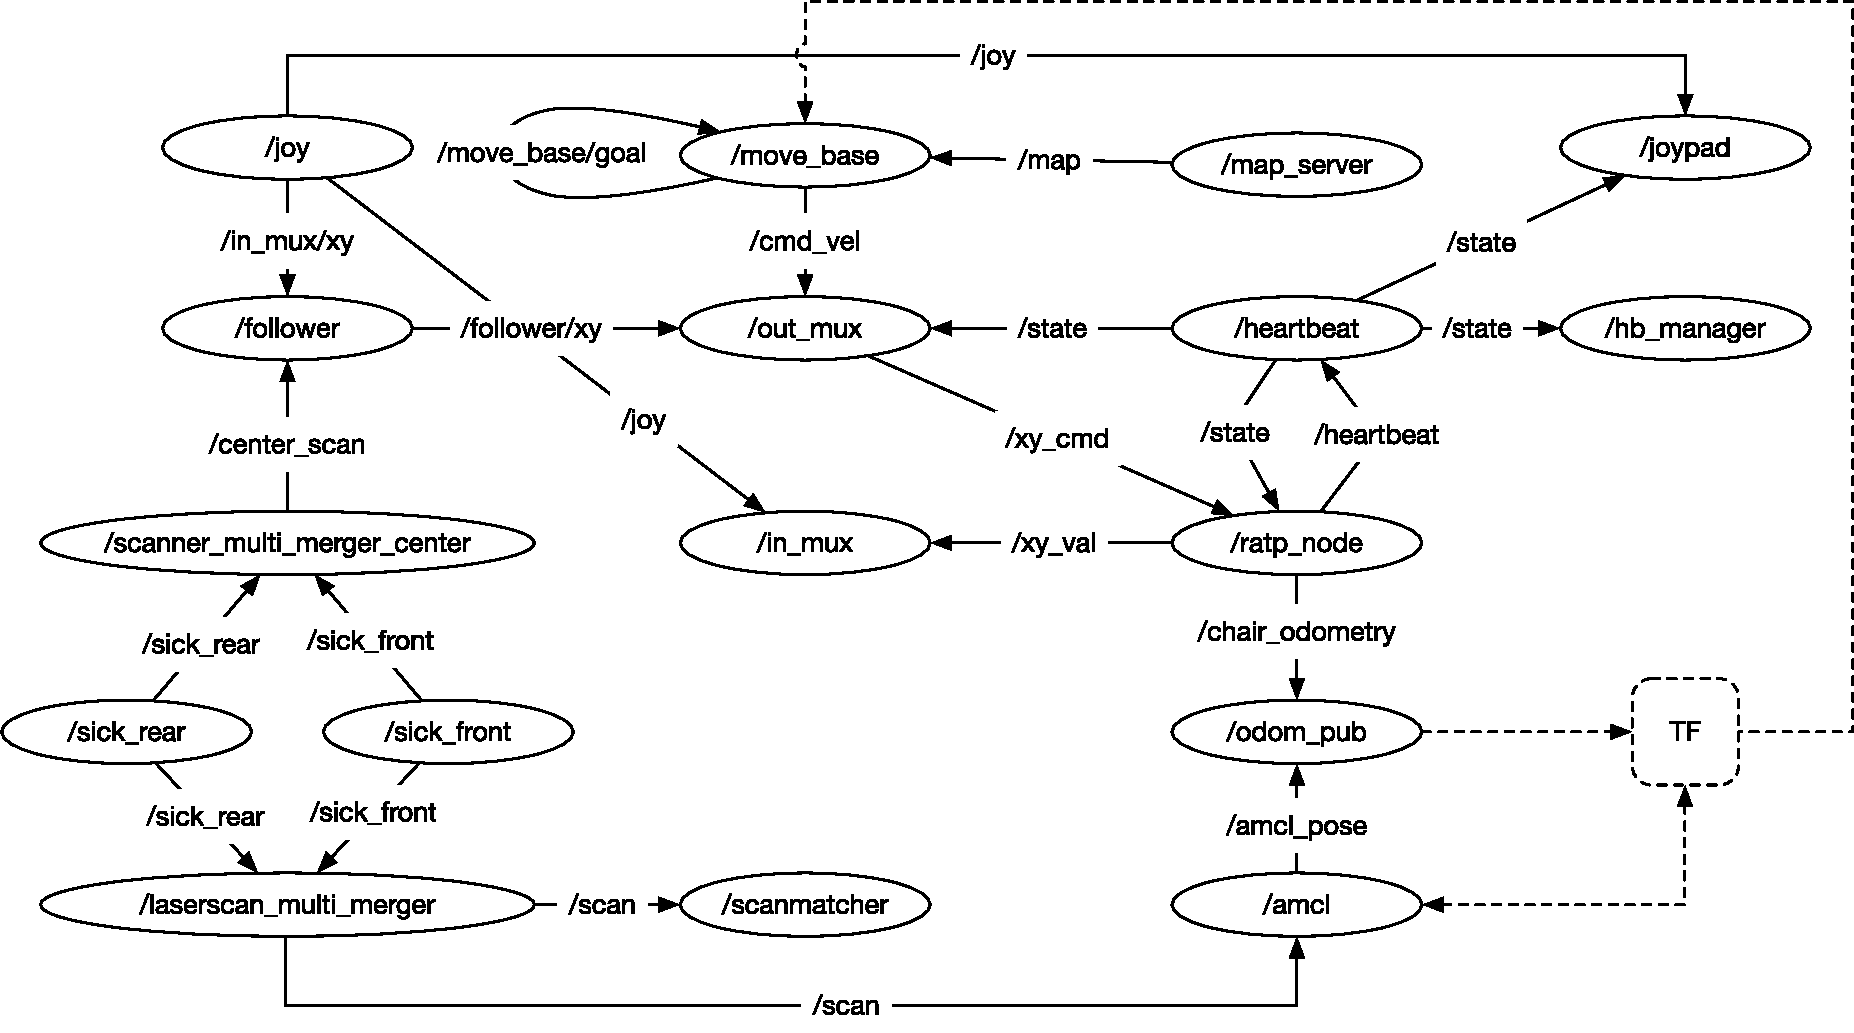
\includegraphics[width=0.95\textheight]{gfx/pmk/hand-graph}
	\caption{TODO}
	\label{fig:pmk-graph}
	\end{figure}
\end{landscape}

\begin{landscape}
	\begin{figure}[t]
	\centering
	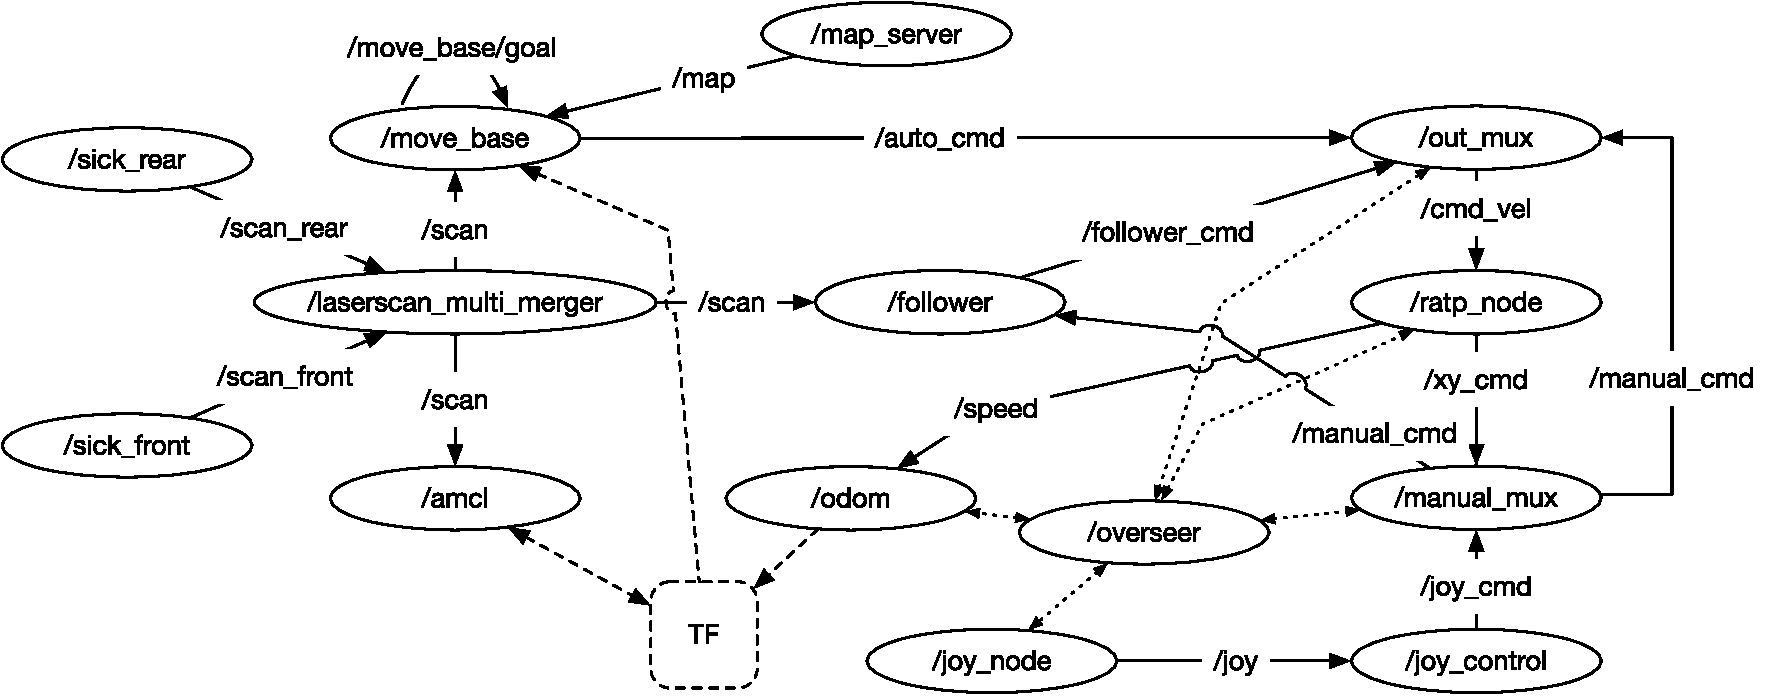
\includegraphics[width=0.95\textheight]{gfx/pmk/gen-graph}
	\caption{TODO}
	\label{fig:gen-graph}
	\end{figure}
\end{landscape}

\begin{figure}[t]
\centering
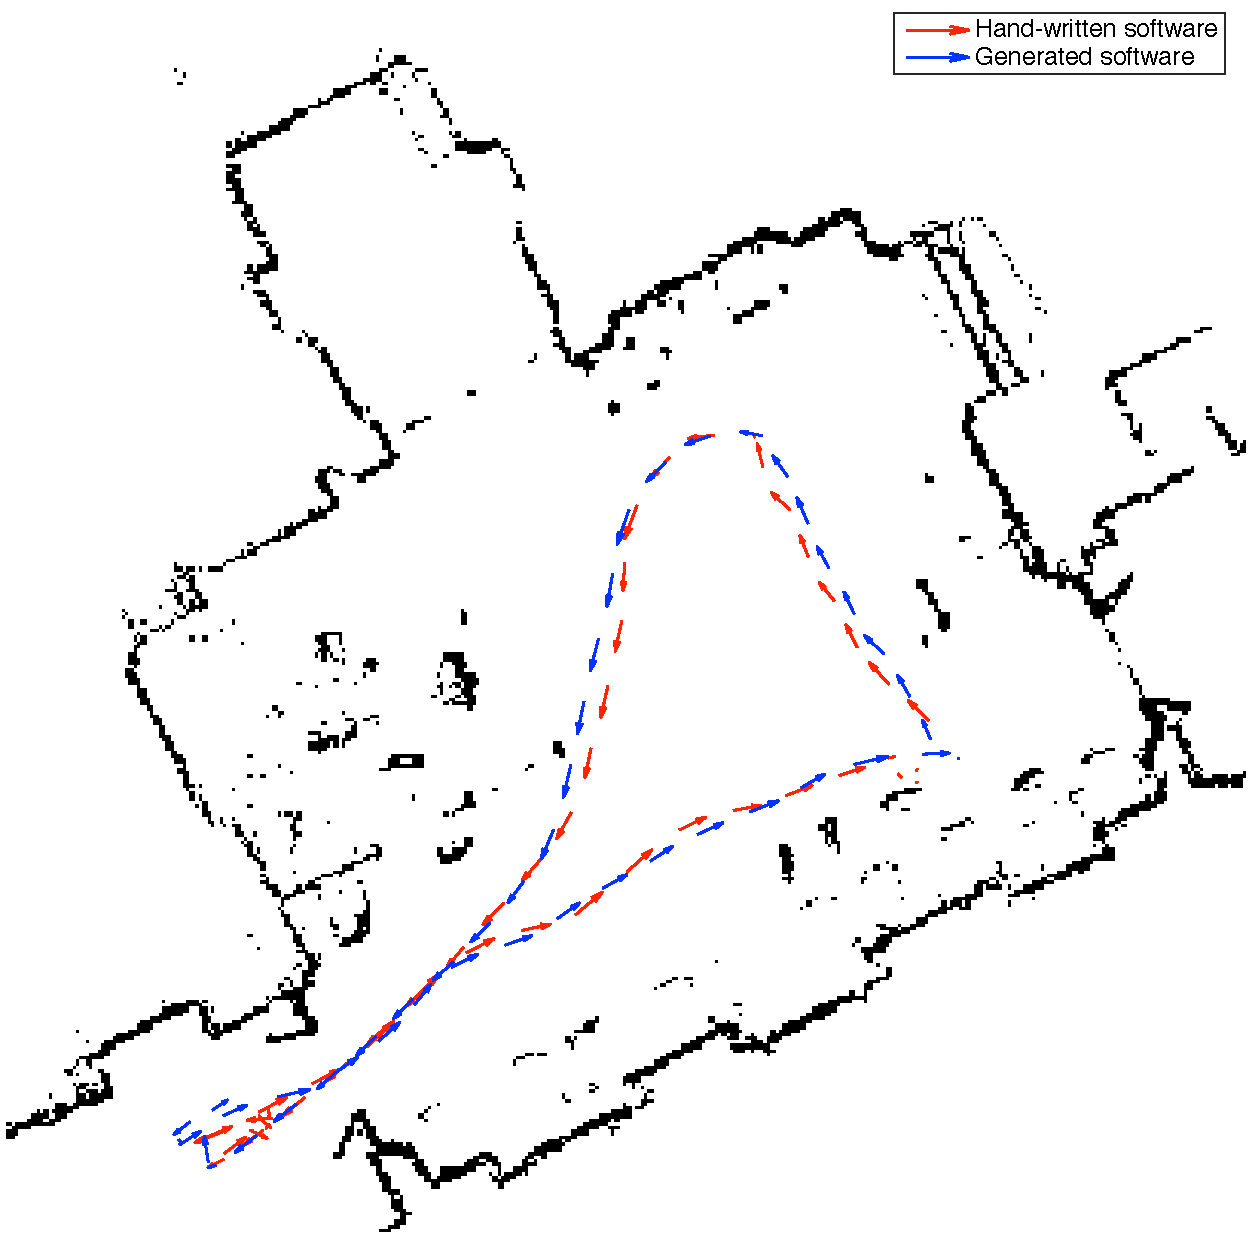
\includegraphics[width=0.95\textwidth]{gfx/pmk/path-followed}
\caption{TODO}
\label{fig:path}
\end{figure}

\subsection{Comparison}
The aim of this use case was to showcase how a complete and functional architecture can be designed and developed entirely using a model-based approach combined with automatic code generation. Starting from an existing architecture was useful for multiple reasons: clear use case and requirements for the robot, existing implementations for all the problem-specific features, precise target functionalities, reference benchmark for the behaviour of the autonomous wheelchair. It was important for us to be able to compare the result of our approach to an existing implementation. In this section, we will analyse the original architecture to show the parallels with the automatic generated one and to highlight existing problems that were solved using a model-based design approach.

First of all, we have to compare the design of the architecture of the wheelchair according to the documentation (Figure~\ref{fig:pmk-doc}) with the runtime computation graph generated by ROS (Figure~\ref{fig:pmk-graph}). With a quick analysis it is possible to see that they do not match, some nodes mentioned in the documentation are not present in the graph (\eg, \textit{dcled\_node}) or vice versa (\eg, \textit{scanner\_multi\_merger\_center}), while others have been replaced (\eg, the standard \textit{map\_server} in place of the custom \textit{map\_server\_pmk}). This is not surprising, the PMK is an ongoing research project where multiple people with varying experience contributed to it. As a result, features were added directly to the codebase without propagating them in the documentation or in the original design. As the project progressed, some of the features were removed, but they left some dangling dependencies behind, in the form of design choices and components. This problem is exacerbated by the fact that ROS does not provide any tool to visualise and analyse the complete architecture before runtime, the only way is to run the entire system and then view the computational graph using tools like \textit{rqt\_graph}. However, even this approach is limited, since it only shows topics, but no services or actions. Of course, a model-based approach does not automatically solve all these problems, since a developer can, and sometimes needs to, directly modify the codebase; however, by combining models and automatic code generation we can create an environment where good practices and designs are encouraged and more natural.

With a deeper analysis of the computational graph it is possible to identify some architectural problems, that were not present in the original design but were introduced in sequential iterations of the project. There are three fundamental issues that could cause unexpected behaviours of the robot.
\begin{itemize}
\item There is a circular dependency between \textit{odom\_pub} and \textit{amcl}. Both nodes are in charge of estimating the position of the robot, the former uses velocity measurement coming from the wheelchair, while the latter matches laser rangefinder data with a know map. The circular dependency happens because each of them expect from the other an initial position to start the estimate. Given how the two algorithms are implemented, an incorrect starting position would not compromise the correct functioning of the system, however it may cause unexpected behaviour, especially after the initial start up of the system.
\item The odometry is estimated twice in the system. This is not directly visible from the graph presented in Figure~\ref{fig:pmk-graph}, since it is not detailed enough, however, the \textit{rapt\_node} pre-compute the odometry of the platform and provide it, together with the velocity measurements, to \textit{odom\_pub}. The initial computation is then discarded and recalculated again directly from the velocity. While this causes no malfunction, it is not a consistent design choice to do a specific processing twice in the same architecture. 
\item The management of the laser scanner measurements is flawed in multiple ways. As explained in Section~\ref{sec:pmk-model}, the navigation subsystem requires an unified source of laser information. In the original documentation, there was a single node in charge of merging the two laser sources, however, in the actual architecture, there are two nodes with the same task: \textit{scanner\_multi\_merger\_center} and \textit{laserscan\_multi\_merger}. Moreover, it is not visible from the computation graph, but the lunch file of the original architecture included a third laser scan merger node,  which it is killed at start up since it has the exact same name of another one, and ROS forbid it. Finally, there is a \textit{scanmatcher} node that subscribe to a topic but has no role in the architecture, a leftover dependency from a removed functionality. Since the duplicated nodes are functionally identical, the overall functionality of the architecture are preserved. However, such a configuration is a waste of computational power and a potential source of significant and dangerous inconsistencies.
\end{itemize}

For comparison, Figure~\ref{fig:gen-graph} shows the computational graph of the architecture resulting from the model-based design and automatic code generation. The overall structure of the system is very similar to the original architecture, however, all the issues identified before have been solved.
\begin{itemize}
\item There is no circular dependency between \textit{amcl} and \textit{odom}. They receive the initial position independently as a parameter or through an external topic.
\item The odometry is estimated only once in the \textit{odom} node. The \textit{ratp\_node} provides directly and only the current speed of the wheelchair as a \textit{Twist} message.
\item Only one node is in charge of unifying the laser sources and the \textit{scanmatcher} node has been removed.
\end{itemize}

Analysing the ROS graph it is useful to provide an overview of the quality of the design of the architecture, however, it gives no insight on the actual functionalities of the system. As seen from the original architecture, design flaws not always translate in a compromised system or faulty behaviours. The robotic wheelchair equipped with the handcrafted architecture supported full autonomous driving with no serious issues, except for minor problems caused by an unstable communication with the low-level control module. This means that we can use the behaviour of the original architecture  to provide an empirical proof of the correctness of the generated architecture. We performed a comparison between the path followed by the wheelchair when running the original system in autonomous mode, and then we gave the same goal to the generated architecture; Figure~\ref{fig:path} shows the result. The resulting paths are extremely similar, this shows that not only the generated architecture replicates the same results of the original one, moreover, all the problem-specific implementations have maintained their original functionalities even after they are transposed in the automatically generated ROS environment.

%*****************************************
